\documentclass[12pt,a4paper]{article}
\usepackage{graphicx}

\usepackage[utf8]{inputenc}
\usepackage[english, spanish]{babel}

\usepackage{wrapfig}
\usepackage{amsmath}
\usepackage{mathtools}
\usepackage{amsfonts}
\usepackage{amssymb}
\usepackage{graphicx}
\usepackage{url}

\usepackage[font=small,format=plain,labelfont=bf,up,textfont=it,up]{caption}
\usepackage{diagbox}
\providecommand{\abs}[1]{\lvert#1\rvert}
\newcommand{\grad}{^{\circ}}

\usepackage[makeroom]{cancel}
\usepackage{enumitem}
\usepackage{float}	
\usepackage{setspace}



\usepackage{subfigure}


\usepackage[export]{adjustbox}

\usepackage{booktabs}
\usepackage{bigstrut}
\usepackage{multirow}
\usepackage{array}
\usepackage{tabularx}
\usepackage{lipsum}  
\usepackage{sectsty}
\usepackage{titlesec}
\usepackage{verbatim}



\usepackage{lscape}
\usepackage{tabu}

\usepackage{array}
\newcolumntype{P}[1]{>{\centering\arraybackslash}p{#1}}

\usepackage{xcolor}
\definecolor{dark}{rgb}{0.10,0.2,0.3}
\definecolor{seablue}{rgb}{0.10,0.2,0.45}
\definecolor{light}{rgb}{1.7,1.5,0.6}
\definecolor{purpure}{rgb}{0.5,0.15,0.3}
\definecolor{bluegreen}{rgb}{0.2,0.65,0.65}
\definecolor{bluegreen2}{rgb}{0.2,0.45,0.45}
\definecolor{vcromo}{rgb}{0.0,0.18,0.39}
\usepackage{hyperref}
\hypersetup{colorlinks,%
citecolor=dark,%
filecolor=dark,%
linkcolor=bluegreen,%
urlcolor=purpure,pdftex}


 
\usepackage[left=3cm,right=3cm,top=2.5cm,bottom=2.5cm]{geometry}

 
\titleformat{\section}[frame]
{\normalfont\sffamily\bfseries\Large\color{vcromo}}{\filcenter\small
\ MEMORIA DE PRÁCTICAS \ }
{10pt}{\LARGE\bfseries\filcenter}

  
\titleformat{\subsection}
  {\normalfont\itshape\large\bfseries\color{dark}}
  {\thesubsection}{1em}{}

\captionsetup[table]{name=Tabla}

%\setcounter{secnumdepth}{5}
%\setcounter{tocdepth}{5}

\providecommand{\abs}[1]{\lvert#1\rvert}
\providecommand{\norm}[1]{\lVert#1\rVert}


\begin{document}
%------Portada--------------%
	\begin{titlepage}
	\centering
    {
\includegraphics[width=0.3\textwidth]{fotos/Logo_azul.png}\par}
	\vspace{1cm}
	{\bfseries\LARGE Universidad Politécnica de Madrid \par}
	\vspace{1cm}
	{\scshape\Large Escuela Técnica Superior de Ingenieros Industriales \par}
	\vspace{2.5cm}
	{\scshape\Huge Programación de Sistemas \par}
	\vspace{0.75cm}
	{\scshape\large Departamento de Electrónica y Automática \par}
	\vspace{2cm}
    {\itshape\LARGE Práctica 1: Diseño de un experimento \par}
    \vspace{0.5cm}
    {\upshape\large Implementación y comparación de un generador dinámico de laberintos en C++ mediante un algoritmo \textit{recursivo} e iterativo}
	\vfill
	{\large{Celia \textsc{Ramos Ramírez} (18295)\par}}
	\vspace{0.1cm}
    {\large{Gonzalo \textsc{Quirós Torres} (17353)\par}}
	\vspace{0.1cm}
	{\large{Josep María \textsc{Barberá Civera} (17048)\par}}
	\vfill
	{\Large{ $3\grad$ \textsc{GITI}}\par}
	\vfill
	{\Large \today \par}
	\end{titlepage}
	
%-----Página en blaco------%
%\newpage
%\begin{center}
%\textit{\{Esta página se ha dejado intencionadamente en blanco\}}
%\end{center}
%\thispagestyle{empty} %	
%\newpage
%------Índice--------------%
%{
%  \hypersetup{linkcolor=black}%Fijaros que estoy cambiando el color solo localmente...es genial para mantener los liks pero que no sea muy cargante el color para el índice de contenidos!!!
%  \tableofcontents
%}

%\pagenumbering{Roman}
%\clearpage

%Si quieres que aparezca en el indice de contenidos pero sin numeración, poner lo siguiente simpre después de algún apartado
%\phantomsection
%\addcontentsline{toc}{subsection}{Manolo el del bombo}

\vspace{-1cm}
\section*{Práctica 1: Determinación de la tensión superficial}

\subsection*{Descripción y objetivos}
Mediante la realización de esta práctica se pretende \textbf{medir la tensión superficial $\sigma$ de un líquido a diferentes temperaturas}. Se utiliza para ello el método de \emph{du Noüy}, en el cual la tensión superficial se determina midiendo la fuerza que hay que emplear para levantar un anillo bañado en el líquido por su cara inferior.
\subsection*{Fundamentos teóricos y del dispositivo}
\begin{wrapfigure}{l}{0.46\textwidth}
\vspace{-0.5cm}
 	 \begin{center}
  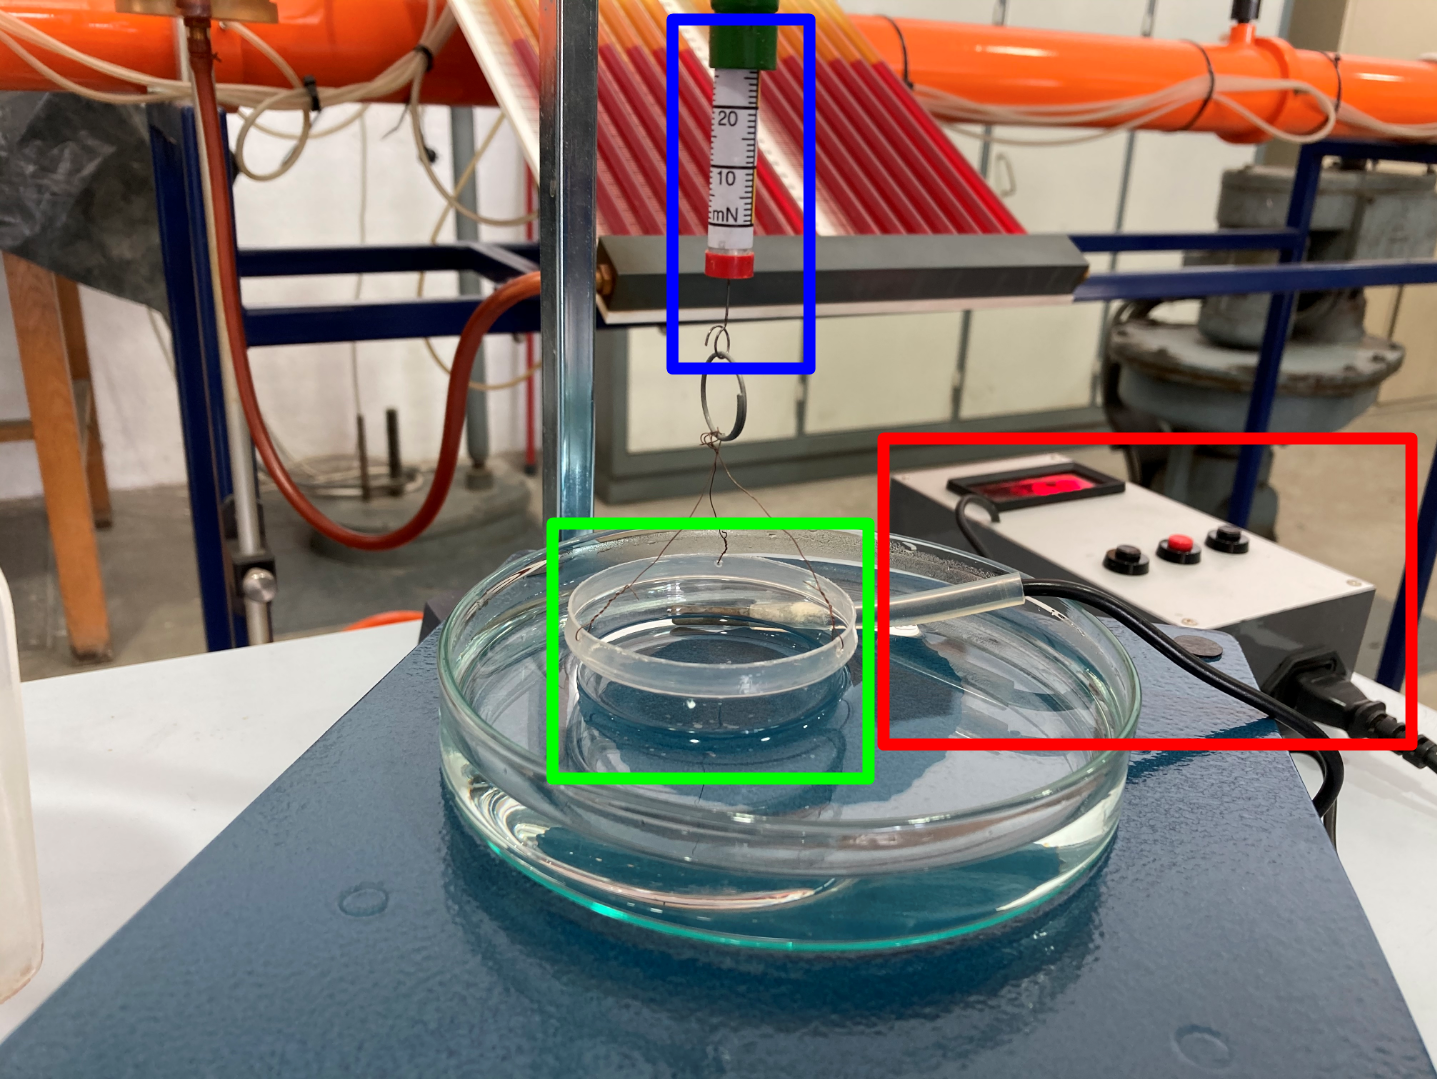
\includegraphics[width=0.44\textwidth]{fotos/tension_superficial_1}
  	 \end{center}
  	\caption{Dispositivo  \emph{du Noüy} para la medida experimental de la tensión superficial.}
  	\label{fig1}
  	
  	\begin{center}
 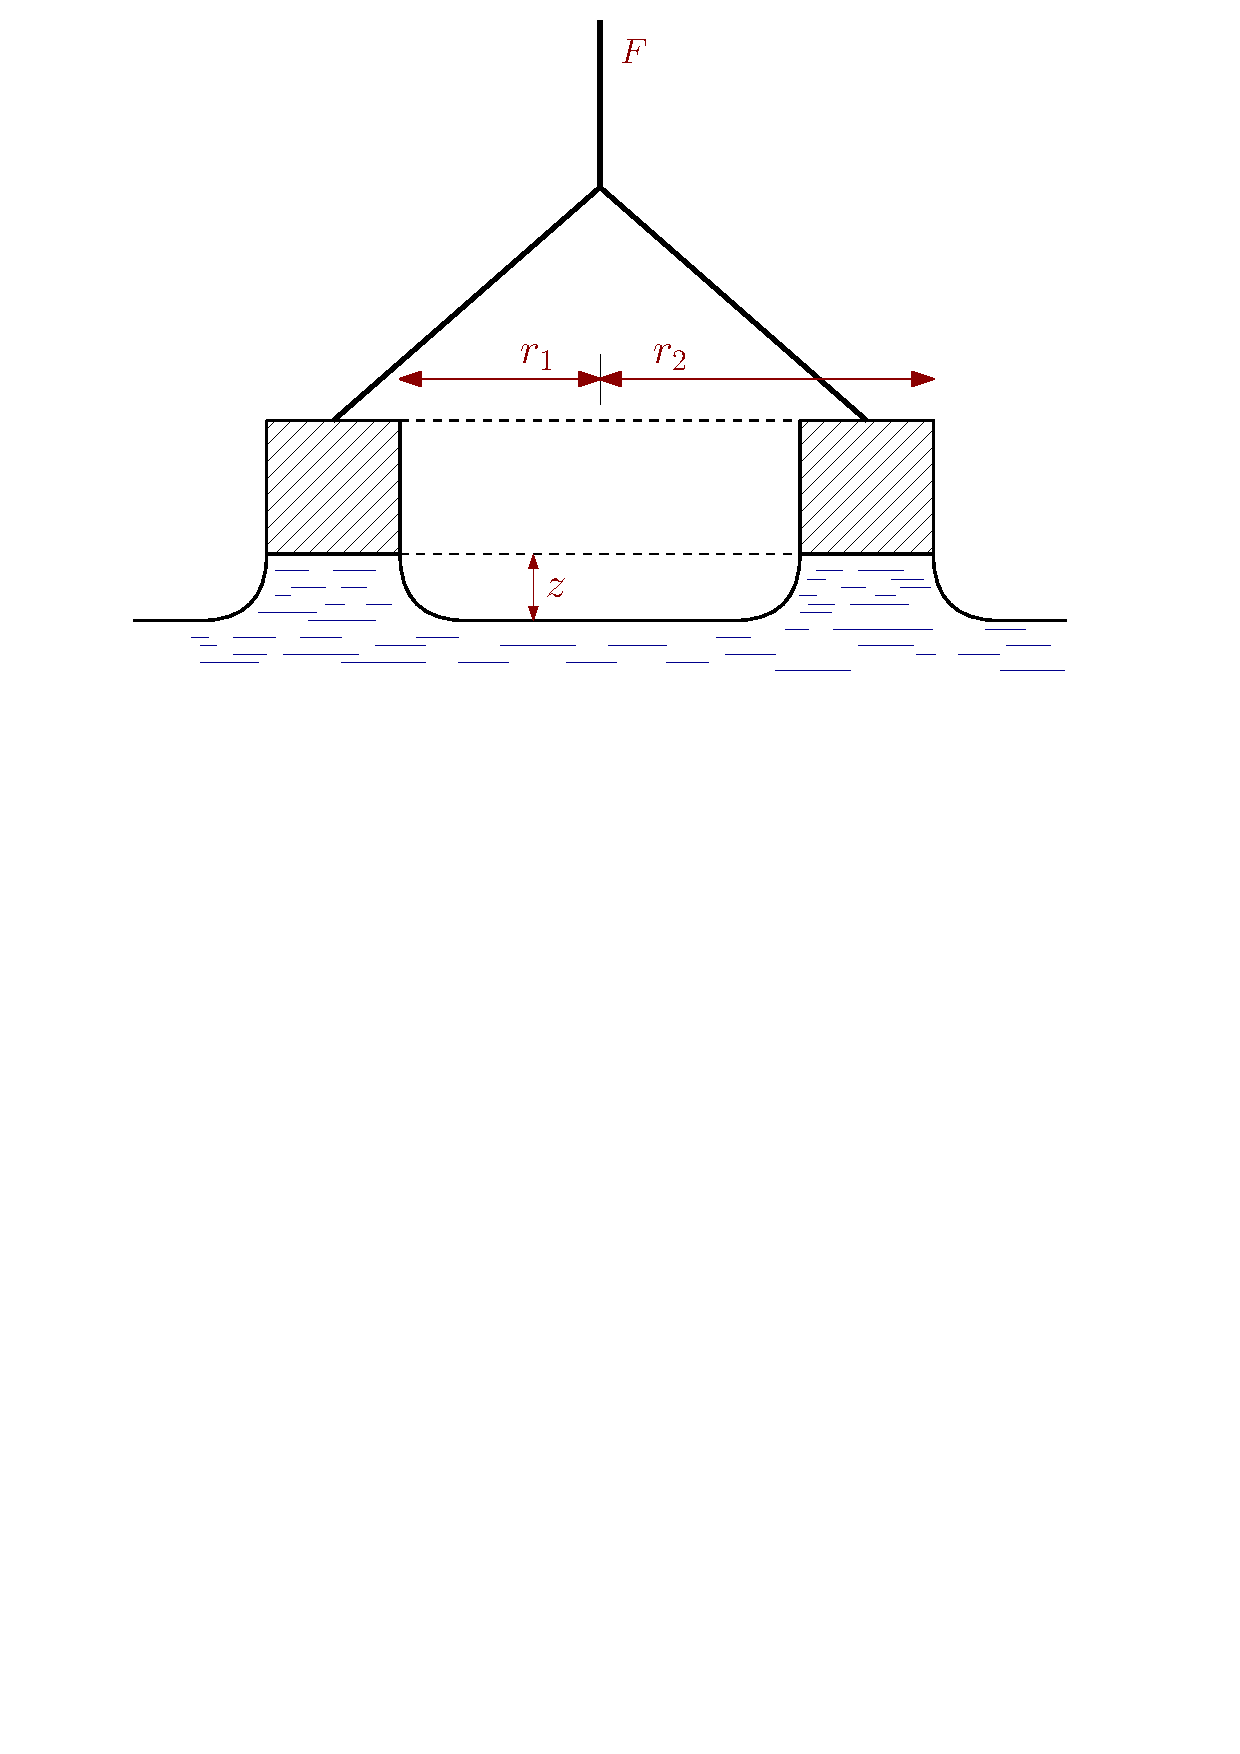
\includegraphics[width=0.44\textwidth]{fotos/esquema_1}
  	\end{center}
  	\caption{Esquema del contacto entre el anillo y el líquido. Realizado mediante \textsl{Ipe drawing editor}}
  	\label{fig2}
\end{wrapfigure}
De forma resumida el experimento se basa en medir con un dinamómetro (en mN) la fuerza que es necesario ejercer para separar el anillo de la superficie del líquido, en nuestro caso agua. Esto se realiza situando de forma vertical un dinamómetro y colgando de este el anillo.
La forma de separar dicho anillo de la superficie del agua es separando la base, en la que se apoya la placa con agua, hacia abajo. Antes de introducir el anillo en el agua, debe medirse (mediante lectura del dinamómetro) el peso del anillo. Este anillo es de plástico y tiene un peso aproximado de $4$ mN, como podrá comprobarse en las tablas que siguen. 

Dicho anillo tiene dos radios, uno exterior de $30\,mm$ y el interior de $29\,mm$, por lo que se pueden aproximar por el radio medio $D=(r_{1}+r_{2})/2=29.5\,mm$, ya que la \emph{longitud capilar} del agua ($\simeq 3\, mm$) es muy superior a la diferencia de radios ($r_{1}-r_{2}=0.5\, mm$). Debe separarse la superficie inferior lentamente hasta que se venza la tensión superficial, anotando el último valor leído en el dinamómetro. Ya se ha comentado el deseo de medir la tensión superficial $\sigma$ a dos rangos de temperaturas, uno a temperatura ambiente ($\simeq\,15 \grad C$) y el otro a mayor temperatura ($\simeq\,45 \grad C$). Se espera, según la teoría que $\sigma$ disminuya al aumentar la temperatura\footnote{En la práctica se ha observado el efecto contrario, suponemos que es debido a una mala medición de la situación en frío. Otra causa posible es la diferente procedencia del agua empleada, siendo un posible experimento realizar dicha práctica con agua de la misma composición.}.

En la \textsc{Fig.}~\ref{fig1} puede verse en rojo el display con el sensor de temperatura y la sonda, en verde el anillo de plástico y en azul el dinamómetro utilizado.
Se incluye a continuación un dibujo esquemático  del anillo de plástico en contacto con el agua, ver \textsc{Fig.}~\ref{fig2}.

Para el cálculo \emph{teórico} de la tensión superficial $\sigma$, se puede emplear la siguiente ecuación:
\begin{align*}
F_{\sigma}=l\cdot \sigma \,\,\,\,\,\, \left[ m\cdot \frac{N}{m}\right]
\end{align*}
donde $l$ es el perímetro del círculo de plástico empleado. No es necesario realizar la suma de los dos perímetros (exterior e interior) pues ya se ha demostrado que se pueden aproximar sus radios por el radio medio, que llamaremos $D$. De esta forma:
\begin{align*}
F_{\sigma}\simeq 2\pi \sigma D
\end{align*}

Se puede demostrar, por otro lado, que en la situación de $r_{1}-r_{2} \ll \lambda_{c}$ la fuerza $F_{\sigma}$ es equivalente a la fuerza total resultante $F$. Es decir, realmente la fuerza total también debería tener en cuenta la fuerza de succión que se produce en el anillo, por la sobrealtura $z$ del agua en contacto con el anillo, pero puede despreciarse por lo anteriormente comentado. Así finalmente podemos afirmar que:
\begin{align*}
F \simeq F_{\sigma} = 2\pi \sigma D \Rightarrow \boxed{\sigma \simeq \frac{F}{2\pi D}}
\end{align*} 
\subsection*{Resultados}

Se incluye a continuación la tabla con los resultados del experimento.
    
\begin{table}[htbp]
  \begin{center}
    \begin{tabular}{cccccc}
    \toprule
    \multicolumn{1}{c}{$\mathbf{T}$} & \multicolumn{1}{c}{$\mathbf{F_{0}}$} & \multicolumn{1}{c}{$\mathbf{F_{1}}$} & \multicolumn{1}{c}{$\mathbf{F}$} & \multicolumn{1}{c}{$\boldsymbol{\sigma}$} & \multicolumn{1}{c}{$\boldsymbol{\sigma}$} \bigstrut[t]\\
    {\small ($\grad C$)} & {\small ($mN$)} & {\small ($mN$)} & {\small ($mN$)} & {\small ($N/m$)} & {\small ($dyn/cm$)}\bigstrut[b]\\
    \midrule
    15 & 4 & 30 & 26 & 0.140 & 140.3 \\
    15 & 4 & 31 & 27 & 0.146 & 145.7 \\
    44 & 4 & 32 & 28 & 0.151 & 151.1 \\
    40 & 4 & 32 & 28 & 0.151 & 151.1 \\
    \bottomrule
    \end{tabular}
    \end{center}
  \caption{Resultados del experimento. Notar que $F=F_{1}-F_{0}$}
  \label{tab1}
\end{table}

Como puede observarse se han tomado cuatro medidas, dos con agua fría y otras dos con agua caliente. En las dos primeras la temperatura era estable y constante. En las últimas el agua se fue enfriando, por eso la diferencia de temperatura entre la tercera y la cuarta medida.
Teóricamente, era de esperar que la tensión superficial disminuyera al aumentar la temperatura, pero en este caso sucede lo contrario. Creemos que esto es debido a otras variables que no se han tenido presentes, como la procedencia, y por tanto, la composición del agua, pues el agua fría y la caliente tenían distinto origen, no eran la misma. Por otro lado, creemos que una posible mejora puede ser aumentar el número de medidas, pudiendo incrementarse hasta tres para cada temperatura, lo cual pondría, quizás, más en evidencia el verdadero carácter de los resultados, pues desconocemos hasta que punto fue el error humano (malas medidas previas, ``contaminación'' del dispositivos, etc.) lo que propició dichos resultados.


\newpage
\section*{Práctica 2: Cálculo del momento hidroestático}
\subsection*{Descripción y objetivos}
En este experimento se pretende \textbf{medir el momento hidroestático sobre un eje}. Para ello se ha empleado el aparato mostrado en la figura \textsc{Fig.}\ref{fig3}. El experimento se realiza con la cara vertical del cuadrante parcial y totalmente sumergida.

\subsection*{Fundamentos teóricos y del dispositivo}
\begin{wrapfigure}{l}{0.5\textwidth}
\vspace{-0.5cm}
 	 \begin{center}
  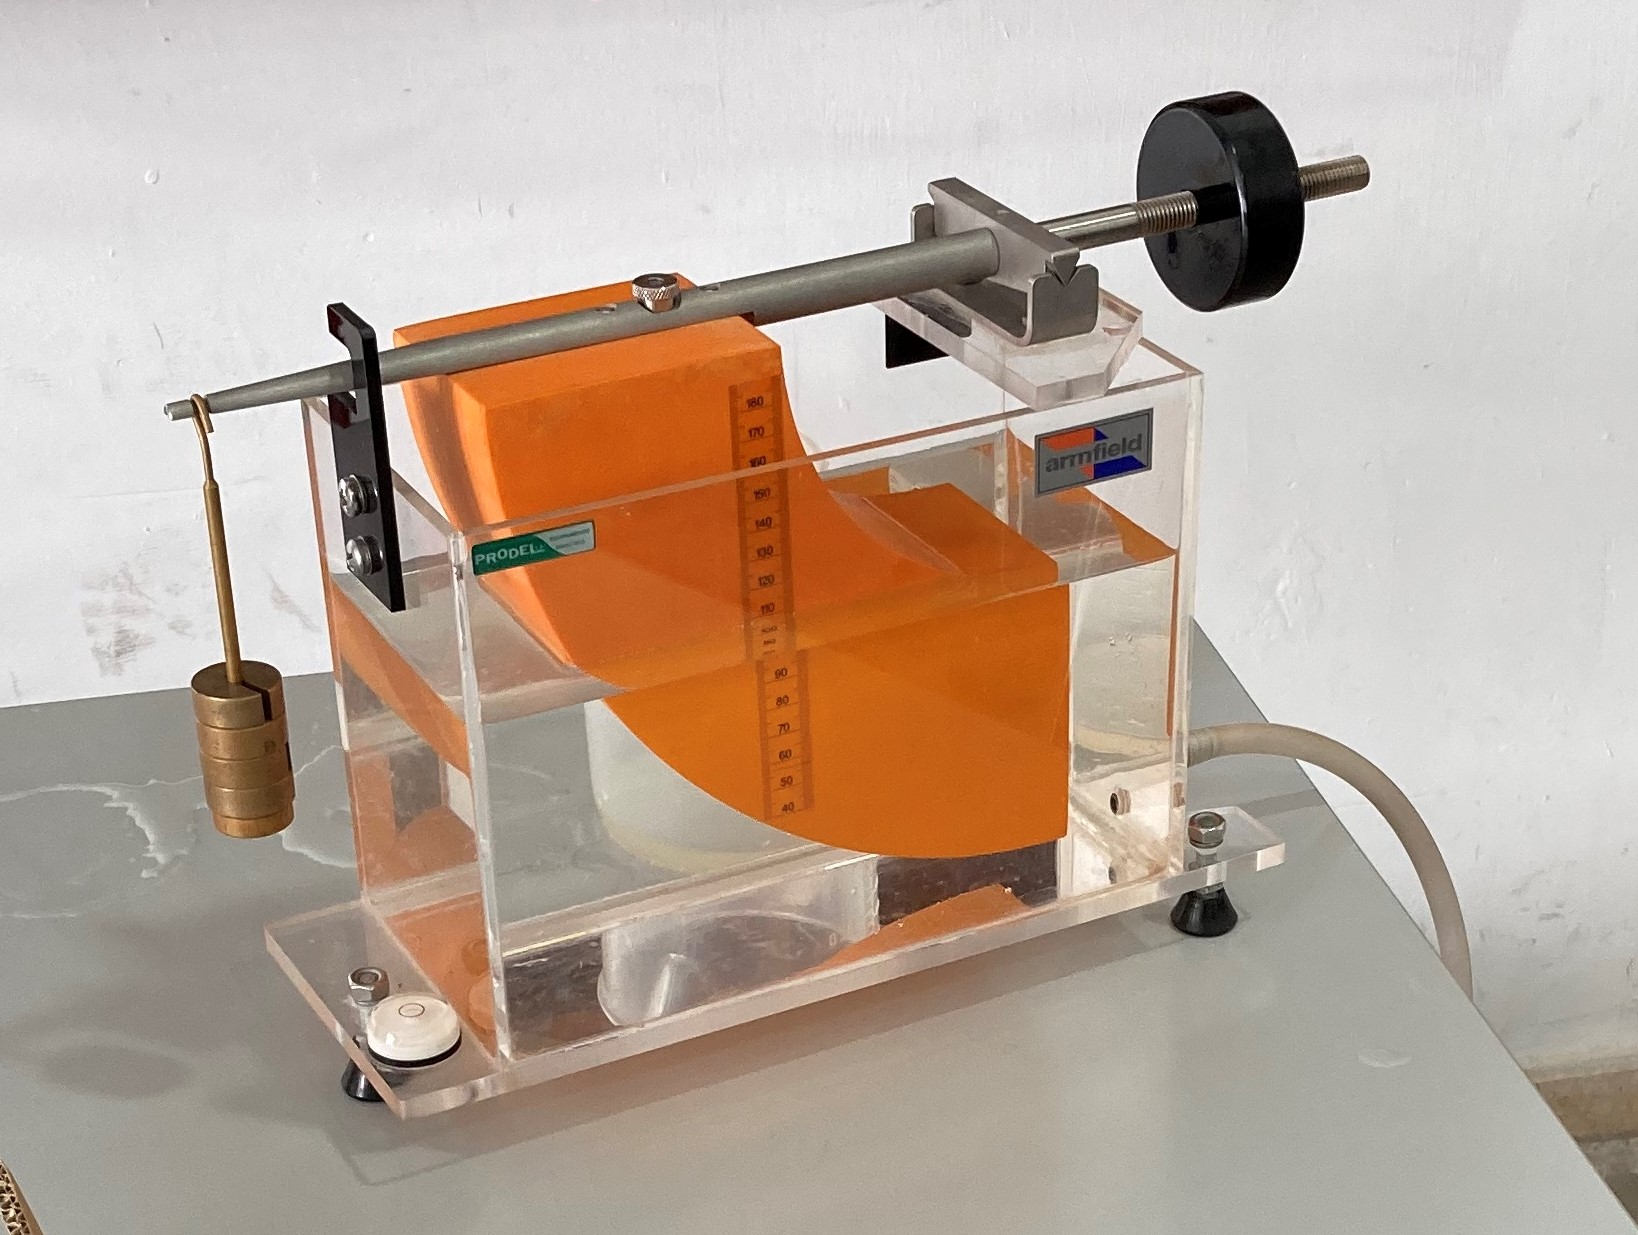
\includegraphics[width=0.48\textwidth]{fotos/momento_hidro}
  	 \end{center}
  	 \vspace{-0.5cm}
  	\caption{Dispositivo experimental para la medida del momento hidroestático}
  	\label{fig3}
  	\vspace{-0.5cm}
\end{wrapfigure}
Se desea medir el momento que realiza el empuje del agua sobre el cuerpo (o cuadrante) naranja sumergido en este. Dicho cuerpo naranja está sujeto a una barra que puede pivotar sobre un eje transversal a la misma (ver círculo rojo en \textsc{Fig.}~\ref{fig4}). Esta barra dispone de dos pesos uno fijo y otro móvil. Además, el fijo puede variar añadiendo pesas (de unos $100$ g cada vez). La forma peculiar del cuerpo naranja se justifica al analizar las fuerza que actúan sobre él y cómo afectan al momento producido sobre el eje de giro. 

Por un lado, las fuerzas laterales son paralelas a dicho eje, por lo que no aportan momento. Por otro lado,  las fuerzas que actúan sobre la parte curva son perpendiculares a su superficie, es decir, con dirección radial según el centro de curvatura de dicha superficie, que coincide con el eje de giro, por lo que tampoco transmiten momento a dicho eje. Finalmente, la única superficie que aporta momento al eje es la cara rectangular vertical del cuadrante.

Al inicio del experimento se equilibran los momentos del peso del cuerpo naranja y de la barra a la que está sujeto con la pesa fija (ver rayado azul en \textsc{Fig.}~\ref{fig4}). Esto se consigue gracias a un indicador de nivel, es decir, se trata de que la barra alcance la posición horizontal. La dinámica del experimento\footnote{Deben tomarse algunas consideraciones y precauciones en la realización del experimento. Lo primero es que el equilibrado inicial debe hacerse sin la varilla que sujete las pesas de $100$g (ver señalado en verde en \textsc{Fig.}~\ref{fig4}). Lo segundo es que al añadir el agua es importante no mojar el cuadrante. Finalmente, comentar la posibilidad de realizar el experimento a la inversa, es decir, en vez de añadir agua retirarla por la llave de descarga.} es la siguiente:   añadir agua al tanque donde está el cuadrante, hasta que el momento hidroestático que resulta de la fuerza de flotación iguale al momento producido por las pesas en cuestión. Medir el valor de la profundidad \emph{d} a la que está sumergido el cuadrante (con la ayuda de la regla impresa sobre el mismo).\\

Con estos datos y la siguiente información es posible calcular los valores del \emph{par experimental} y del \emph{par teórico}, para posteriormente calcular el \emph{error relativo} entre ambos.

\begin{figure}[H]
\vspace{-0.2cm}
 	 \begin{center}
  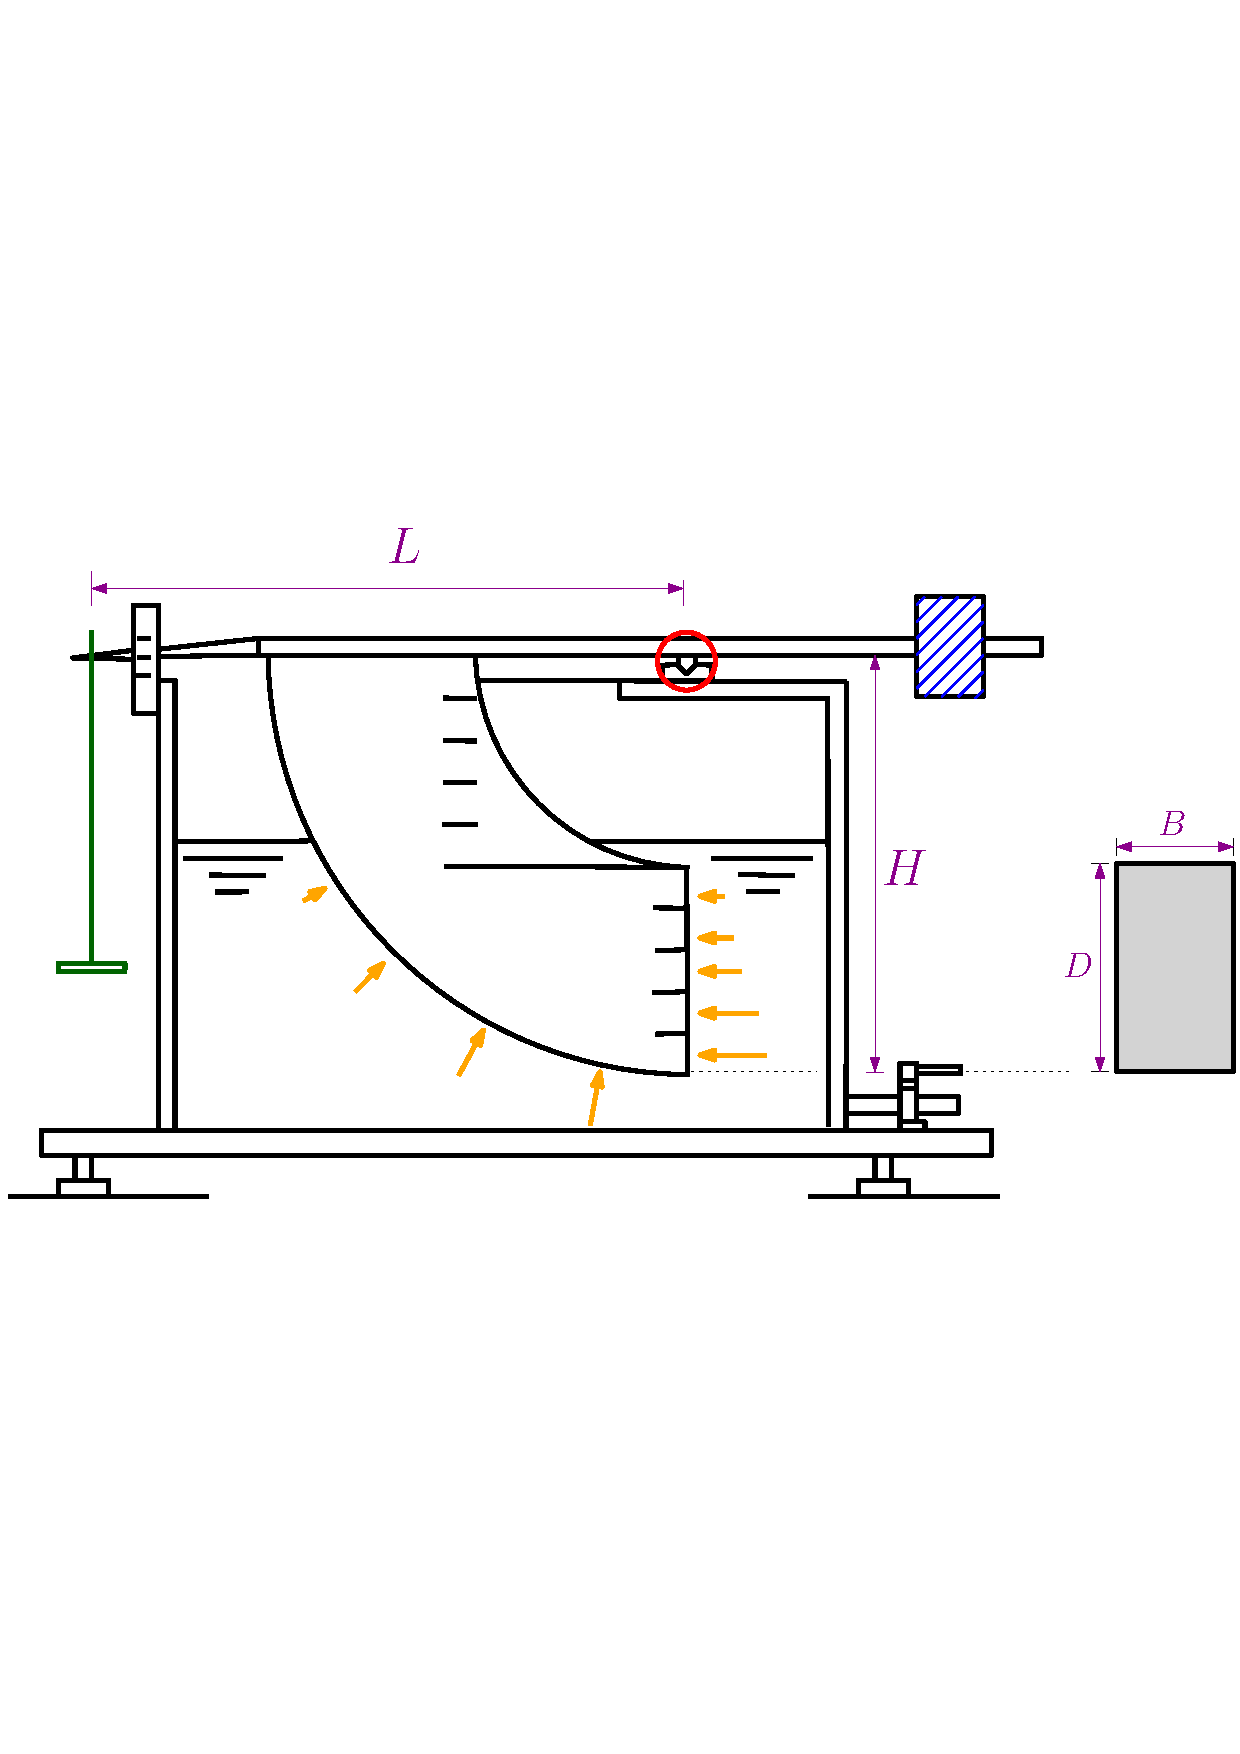
\includegraphics[width=0.9\textwidth]{fotos/esquema_2}
  	 \end{center}
  	\caption{Gráfico del aparato utilizado en prácticas. Se han señalado en otro color elementos importantes así como las fuerzas que actúan sobre el cuadrante. Los valores necesarios para los cálculos que siguen son: $L=0.275\,m$, $B=0.075\,m$, $D=0.1\,m$ y $H=0.2\,m$.}
  	\label{fig4}
  	\vspace{-0.2cm}
\end{figure}

Los valores del \emph{par experimental} y del \emph{par teórico} pueden calcularse mediante las siguientes fórmulas (para más información consultar el guión de prácticas):

\begin{align*}
T_{TS}&= \rho g B \left( \frac{d^{3}-(d-D)^{3}}{3} + (H-d)\frac{d^{2}-(d-D)^{2}}{2}\right)\\
T_{PS} &= \rho g B \left( \frac{d^{3}}{3} + (H-d) \frac{d^{2}}{2}\right)
\end{align*}
donde los subíndices $TS$ y $PS$ hacen referencia a \emph{Totalmente Sumergido} y \emph{Parcialmente Sumergido} respectivamente, del par teórico.
Por otro lado el par experimental se calculará sabiendo la masa $m$ situada en la varilla porta masas, de la siguiente forma: $$ \boxed{T_{e}=m g L}$$

\subsection*{Resultados}
Incluimos a continuación la tabla con los resultados obtenidos en el experimento. Por ser más visual e intuitivo se ha expresado el valor de los pares experimentales y teóricos en $mN\,m$. Por otro lado, se ha calculado el error relativo como el valor absoluto de la diferencia entre el par experimental y el par teórico dividido por el valor teórico en tanto por ciento.
\vspace{-0.3cm}
\begin{table}[htbp]
  \centering
    \begin{tabular}{ccccc}
    \toprule
    \multicolumn{1}{c}{$\mathbf{m}$} & \multicolumn{1}{c}{$\mathbf{d}$} & \multicolumn{1}{c}{$\mathbf{T_{e}}$} & \multicolumn{1}{c}{$\mathbf{T_{t}}$} & \multicolumn{1}{c}{$\boldsymbol{\left| \frac{T_{e}-T_{t}}{T_{t}} \right|}$} \\
      {\small ($g$)} & {\small ($mm$)} & {\small ($mN{\cdot}m$)} & {\small ($mN{\cdot}m$)} & {\small ($\%$)} \\    
    \midrule    
    50 & 46 & 134.9 & 143.7 & 6.16 \\
    100 & 65 & 269.8 & 277.2 & 2.67 \\
    150 & 81 & 404.7 & 417.6 & 3.09 \\
    200 & 96 & 539.6 & 569.6 & 5.27 \\
    250 & 110 & 674.4 & 723.5 & 6.78 \\
    300 & 120 & 809.3 & 833.9 & 2.94 \\
    350 & 127 & 944.2 & 911.1 & 3.63 \\
    400 & 145 & 1079.1 & 1109.8 & 2.76 \\
    450 & 157 & 1214.0 & 1242.2 & 2.27 \\
    \bottomrule
  \end{tabular}
   \caption{Resultados del experimento. Es necesario indicar que la expresión utilizada en el cálculo del par teórico cambia si la medida de \emph{$d$} pasa por encima de $100\, mm$. Notar también que $T_{t}$ es el par teórico y que engloba tanto a $T_{TS}$ como a $T_{PS}$.}
  \label{tab2}
\end{table}

\begin{figure}[H]
 	 \begin{center}
  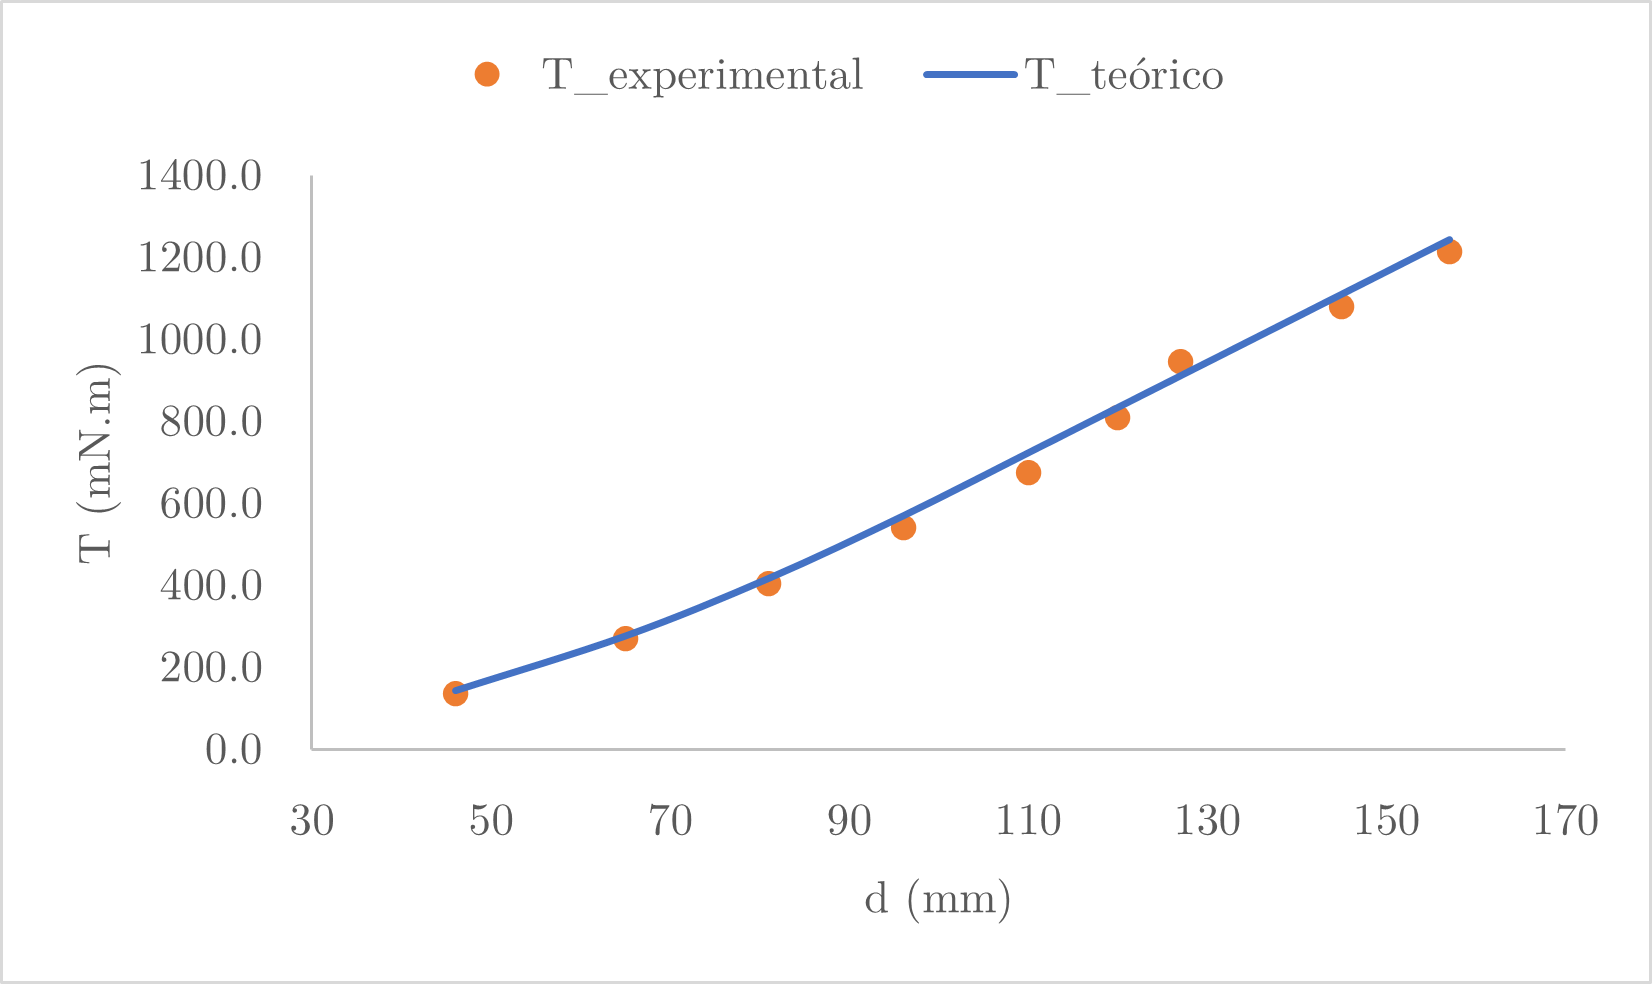
\includegraphics[width=0.9\textwidth]{fotos/grafico_2}
  	 \end{center}
  	 \vspace{-0.3cm}
  	\caption{Par teórico ($T_{t}$) en azul y par experimental ($T_{e}$) en naranja frente a $d$.}
  	\label{fig5}
  	\vspace{-0.2cm}
\end{figure}

Puede comprobarse primero en la tabla \ref{tab2} y luego en la en el gráfico \ref{fig5} como los valores teóricos y los experimentales son parecidos. El valor máximo del error ocurre con la masa de $250\,g$ y el valor mínimo con la masa de $450\,g$. 

Puede concluirse así que el cálculo teórico responde bien a la realidad. El experimento resulta fiable, con la salvedad de la difícil lectura del valor $d$. Creemos que se encuentra allí todo el error experimental. Este puede subsanarse midiendo simplemente el nivel del agua con una regla adherida en el interior del depósito, pues conocidas las dimensiones del aparato y sabiendo qué posición supone el equilibrio, solo es necesario saber el nivel del agua. Igual que es conocido el valor $H$, también podría conocerse la misma altura hasta la base del depósito. La diferencia entre $H$ y este valor (que llamaremos $S$) sería la altura a la que está la parte inferior del cuerpo naranja respecto de la base del depósito. Conocida la altura del agua ($N$), $d$ sería simplemente: $d=N-(S-H)$.



\newpage
\section*{Práctica 3: Cálculo de la superficie libre de un líquido en rotación}

\subsection*{Descripción y objetivos}
Mediante la realización de esta práctica se pretende \textbf{medir de forma experimental la superficie libre de un fluido líquido en rotación contenido en un depósito cilíndrico}. Se medirán físicamente algunos parámetros característicos (que se explican en el siguiente apartado) y se compararán dichos datos con los calculados teóricamente, para ver cuánto y de qué forma coinciden.

\subsection*{Fundamentos teóricos y del dispositivo}
Tomando el sistema de referencia conveniente, el estudio deseado puede considerarse el de un líquido en reposo. En este caso la ecuación que modela dicho comportamiento para un líquido es:
\begin{align*}
\rho\, U+p=cte
\end{align*}
donde $U$ es el potencial del cual derivan las fuerzas másicas. En nuestro caso de aplicación el potencial viene dado por la siguiente expresión:
\begin{align}
U=gz-\frac{1}{2}\omega^2 r^2
\label{eq1}
\end{align}

\begin{wrapfigure}{l}{0.5\textwidth}
\vspace{-0.5cm}
 	 \begin{center}
  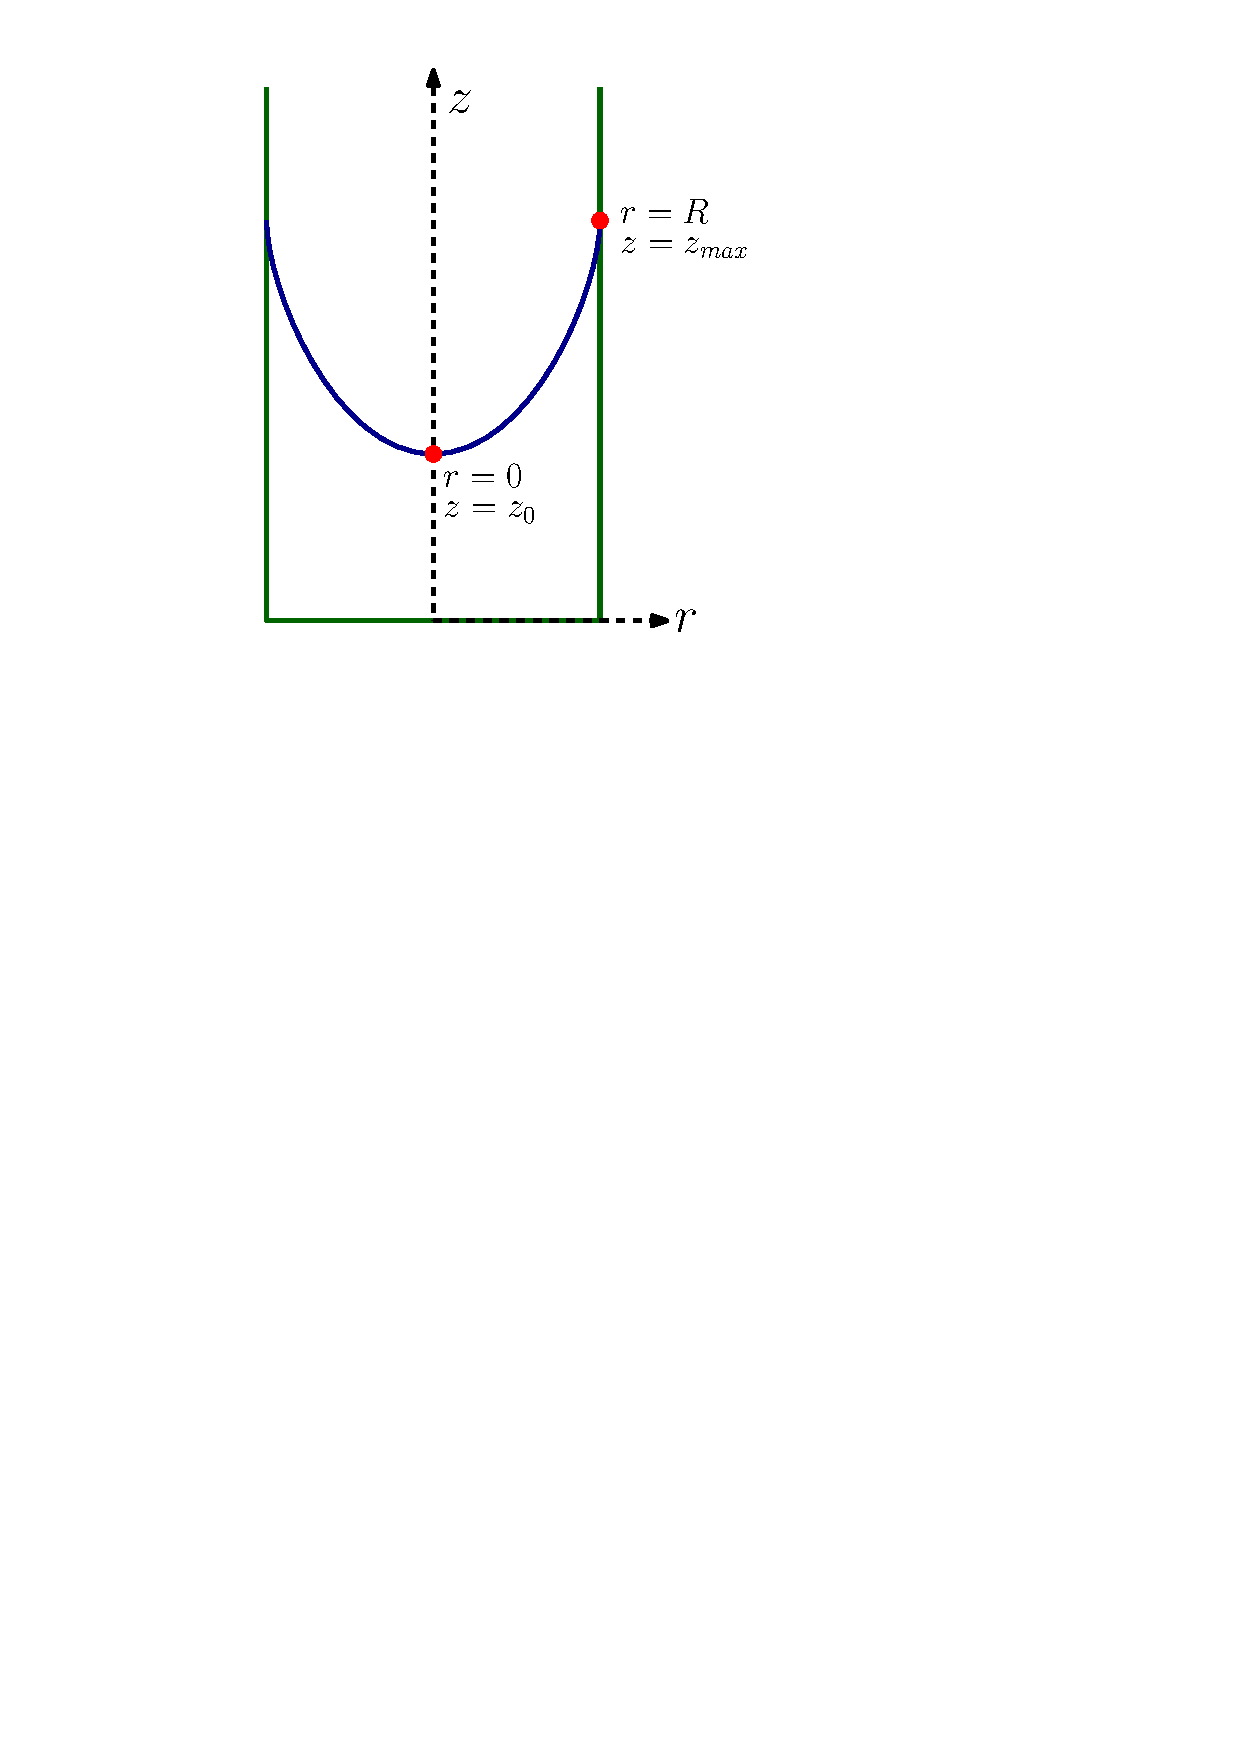
\includegraphics[width=0.48\textwidth]{fotos/esquema_3}
  	 \end{center}
  	 \vspace{-0.5cm}
  	\caption{Esquema de la superficie libre y sus puntos carácterísticos.}
  	\label{fig6}
  	\vspace{-0.5cm}
\end{wrapfigure}

Es decir, actúa la gravedad y una fuerza centrífuga $\omega$.
Es estas condiciones por ser la presión (atmosférica) contante en la superficie del líquido sabemos que $U$ también será constante en dicha superficie libre. Lo cual nos lleva a asegurar que tanto en el punto más bajo de dicha superficie como en el más alto $U$ será constante (aplicando esto en la ecuación \ref{eq1}):
\begin{align*}
U(r=0,z=z_{0})= & U(r=R,z=z_{max})\\
gz_{0}-0= & gz_{max}-\frac{1}{2}\omega^2 R^2
\end{align*}
Finalmente, despejando la diferencia de alturas:
\begin{align*}
z_{max}-z_{0}=\frac{\omega^2 R^2}{2g}
\end{align*}


Esta diferencia de alturas $\Delta z$ (la elevación del líquido desde su punto más bajo hasta su punto más alto) puede expresarse también de la siguiente forma si tenemos en cuenta que $R=\frac{D}{2}$:
\begin{align}
\boxed{\Delta z =\frac{\omega^2 D^2}{8g}}
\label{eq2}
\end{align}

\vspace{-0.3cm}
\subsection*{Resultados}

\begin{wrapfigure}{l}{0.36\textwidth}
\vspace{-0.6cm}
 	 \begin{center}
  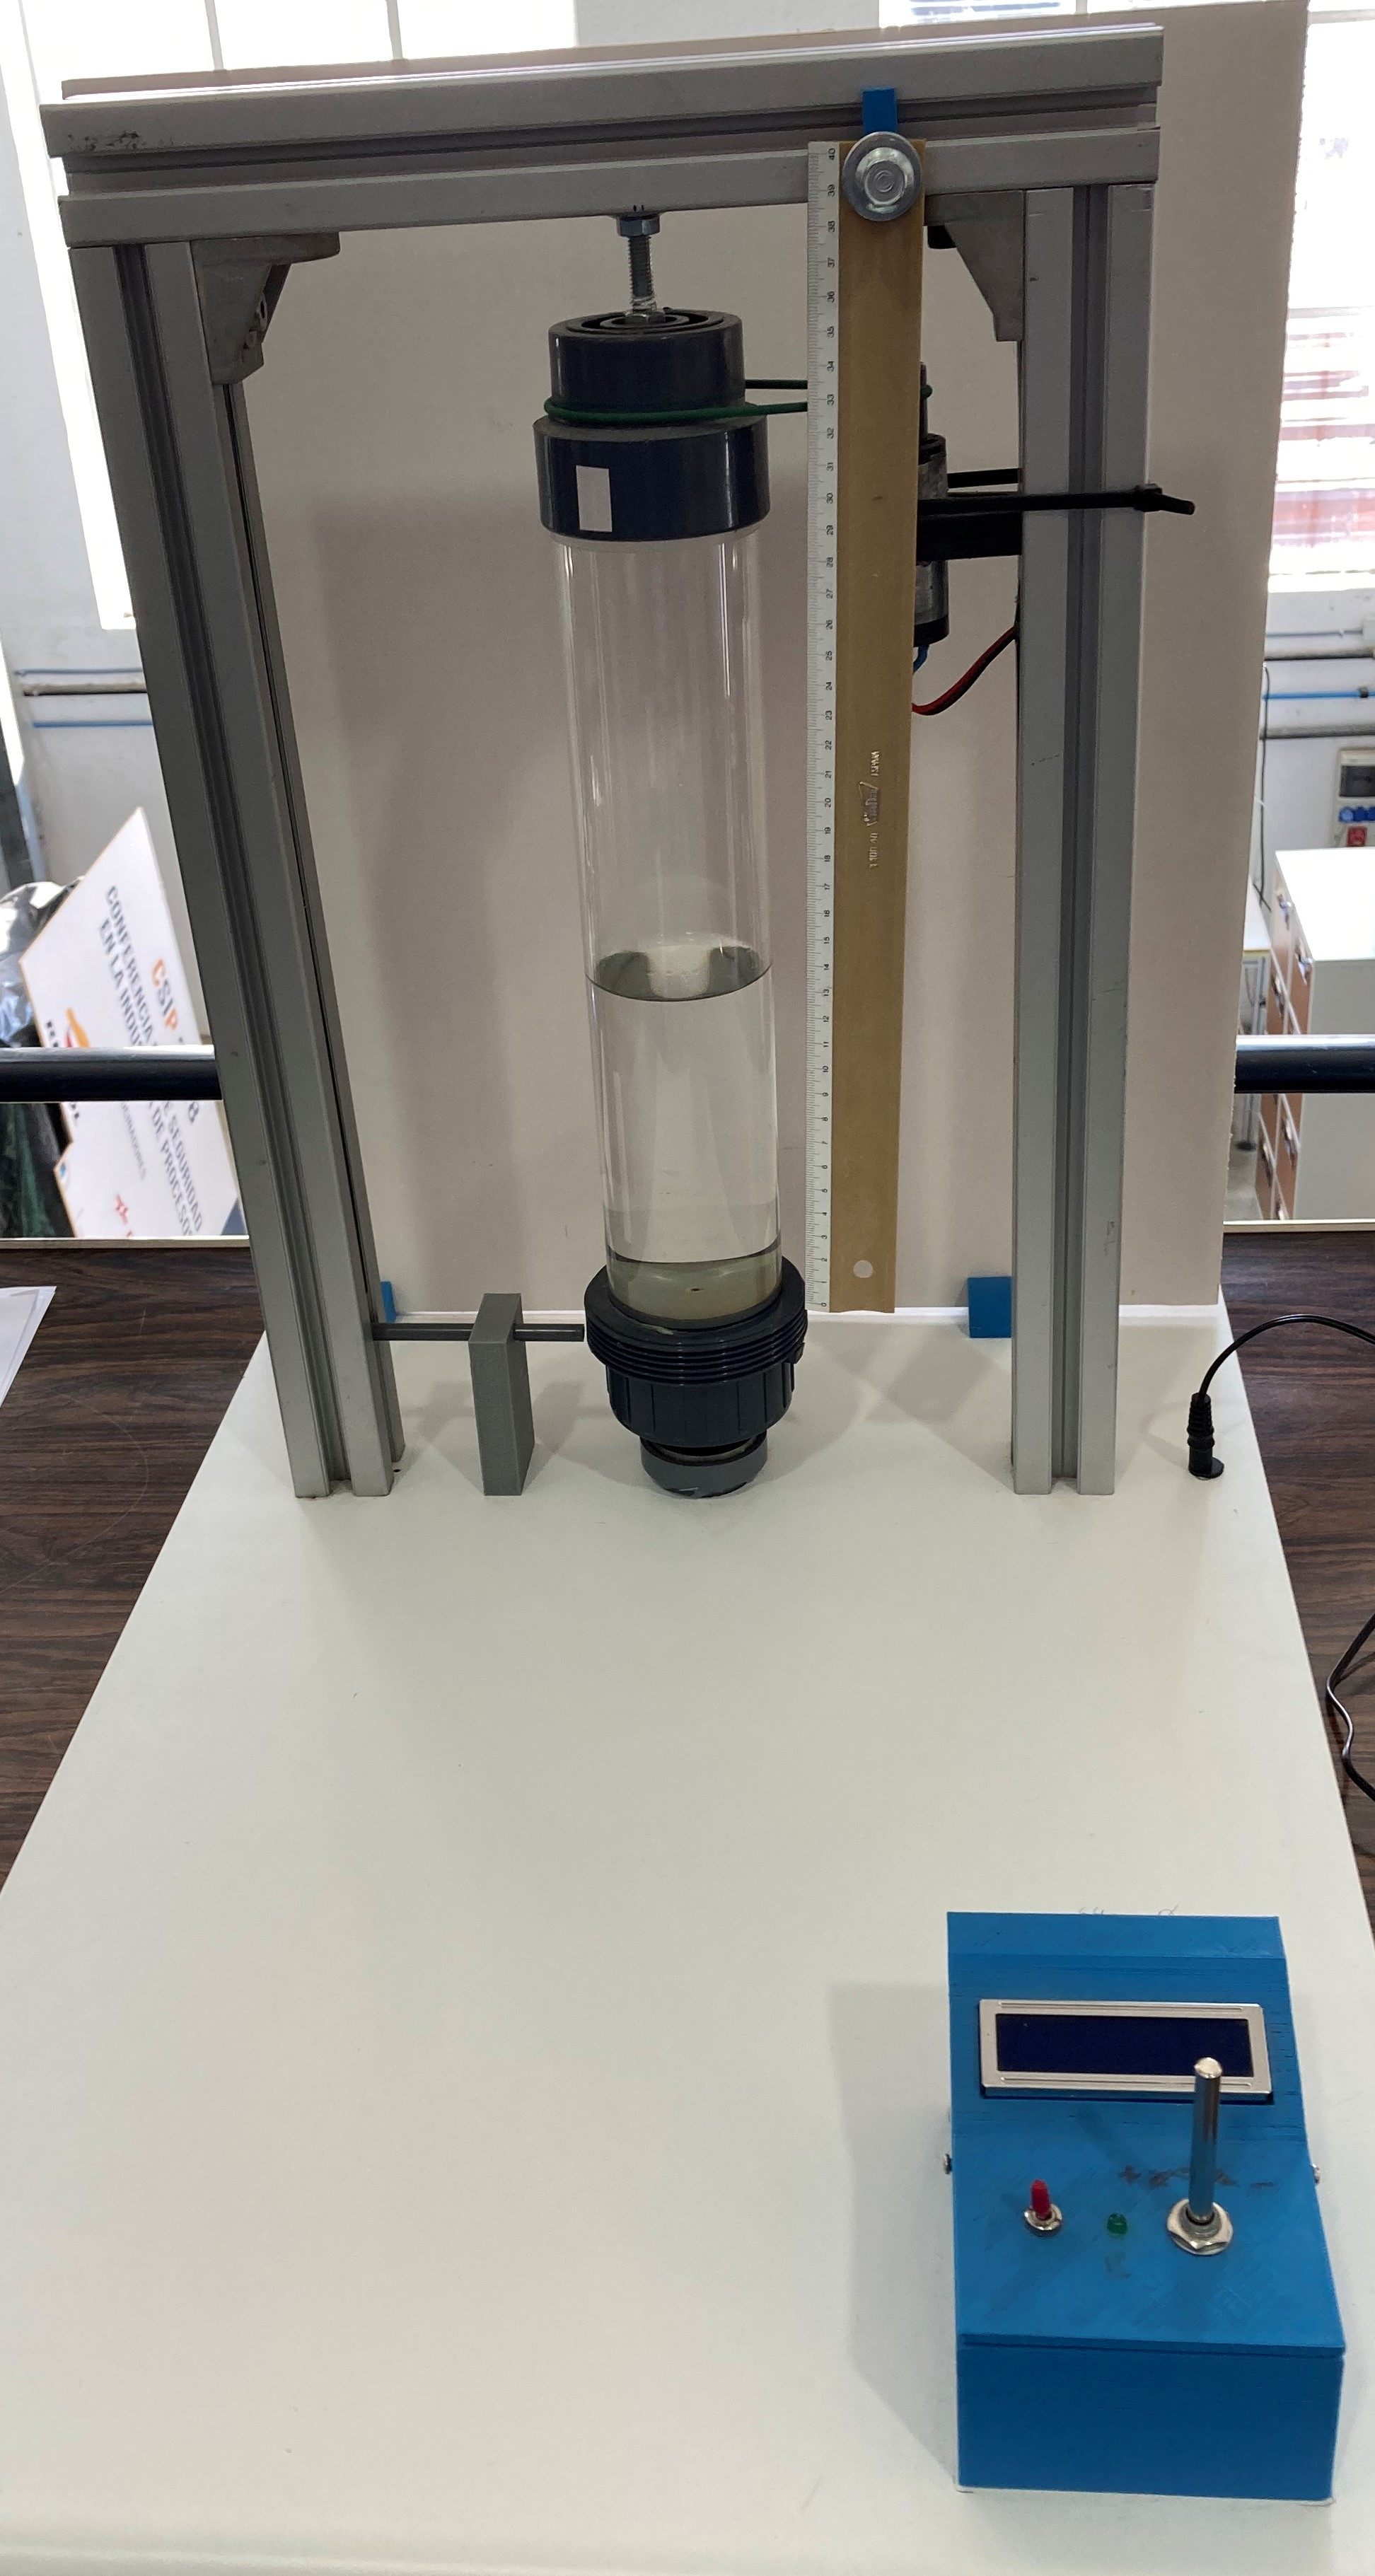
\includegraphics[width=0.34\textwidth]{fotos/aparato_3}
  	 \end{center}
  	 \vspace{-0.5cm}
  	\caption{Dispositivo empleado.}
  	\label{fig7}
\end{wrapfigure}

Se incluye aquí una fotografía del aparato utilizado en la práctica. 
Puede observarse un panel azul con el interruptor de encendido, un piloto rojo y una varilla que regula mediante un potenciómetro la velocidad $w$. También dispone de un display que muestra la velocidad en $rpm$. Toda la carcasa ha sido impresa mediante impresora 3D, muy posiblemente en las instalaciones de la escuela. Por otro lado, el control de velocidad y encendido se realiza mediante un microcontrolador, del tipo \emph{Arduino}.

La metodología empleada fue la siguiente, mediante el cuadro de control se ponía en funcionamiento el dispositivo y se aumentaba la velocidad hasta llegar a la deseada. Después  era necesario dejar al sistema estabilizarse  y finalmente, con la ayuda de una regla dispuesta verticalmente (como se puede observar en la figura \ref{fig7}) se media tanto $z_{0}$ como $z_{max}$.

Se pone a continuación la tabla con los datos obtenidos y los calculados de forma teórica con la ecuación \ref{eq2}:

\begin{table}[htbp]
  \centering
    \begin{tabular}{ccccccc}
    \toprule
    \multicolumn{1}{c}{$\mathbf{n}$} & \multicolumn{1}{c}{$\mathbf{w}$} & \multicolumn{1}{c}{$\mathbf{z_{0}\,exp.}$} & \multicolumn{1}{c}{$\mathbf{z_{max}\,exp.}$} & \multicolumn{1}{c}{$\boldsymbol{\Delta z \,exp.}$} & \multicolumn{1}{c}{$\boldsymbol{\Delta z\,te\acute{o}r.}$} & \multicolumn{1}{c}{$\mathbf{\left|\frac{\Delta z_{e}-\Delta z_{t}}{\Delta z_{t}}\right|}$} \\
    {\small ($rpm$)} & {\small ($rad/s$)} & {\small ($cm$)} & {\small ($cm$)} & {\small ($cm$)} & {\small ($cm$)} & {\small ($\%$)}\\
    \midrule
    240 & 25.13 & 11.5 & 14.8 & 3.3 & 3.297 & 0.10 \\
    300 & 31.42 & 10.9 & 15.8 & 4.9 & 5.15 & 4.87 \\
    360 & 37.70 & 9.7 & 16.4 & 6.7 & 7.42 & 9.67 \\
    420 & 43.98 & 8.4 & 17.6 & 9.2 & 10.10 & 8.88 \\
    480 & 50.27 & 7.3 & 18.5 & 11.2 & 13.19 & 15.07 \\
    510 & 53.41 & - & - & 12.5 & 14.89 & 16.03 \\
    540 & 56.55 & 4.8 & 20.6 & 15.8 & 16.69 & 5.33 \\
    570 & 59.69 & - & - & 17 & 18.60 & 8.58 \\
    600 & 62.83 & 4 & 22.1 & 18.1 & 20.60 & 12.15 \\
    630 & 65.97 & - & - & 20.5 & 22.72 & 9.76 \\
    \bottomrule
    \end{tabular}
    \caption{Resultados del experimento. Notar que faltan datos en algunas filas, esto se debe a que quien recogió dichos datos apuntó directamente la diferencia de alturas y no los datos de $z_{0}$ y $z_{max}$ por separado.}
  \label{tab3}
\end{table}
\newpage

\begin{figure}[H]
 	 \begin{center}
  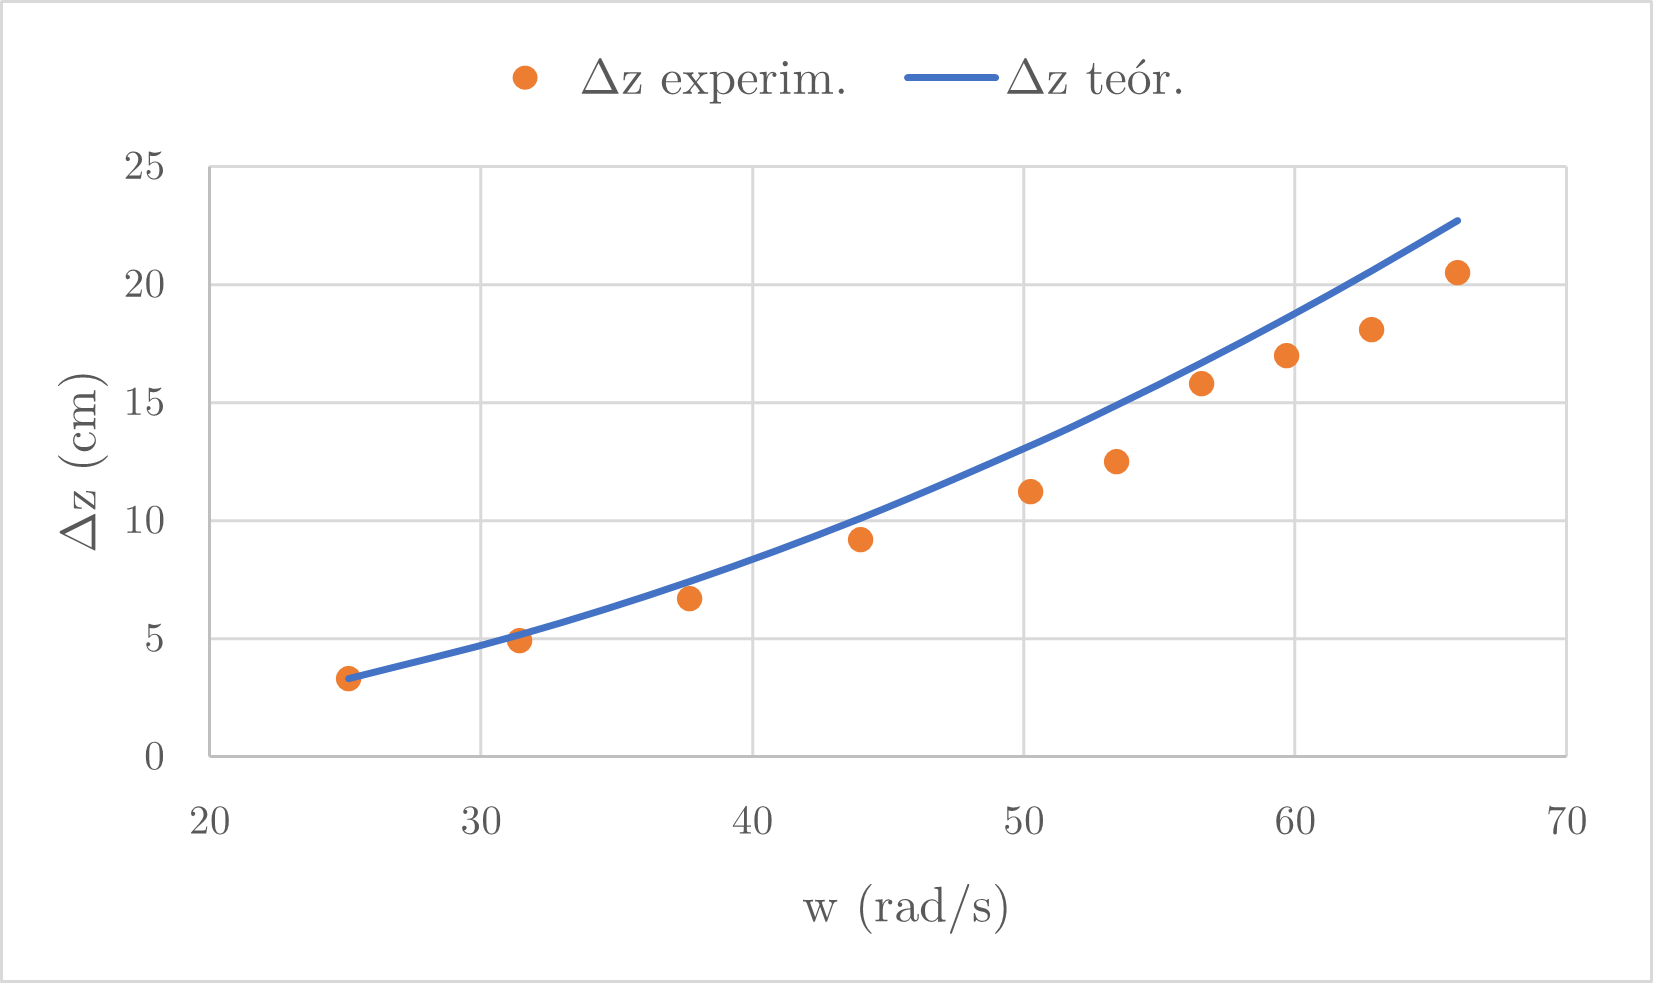
\includegraphics[width=0.9\textwidth]{fotos/grafico_3}
  	 \end{center}
  	 \vspace{-0.3cm}
  	\caption{Diferencia de altura teórica ($\Delta z_{t}$) en azul y diferencia teórica experimental ($\Delta z_{e}$) en naranja frente a $w$.}
  	\label{fig8}
  	\vspace{-0.2cm}
\end{figure}

A la vista de la figura \ref{fig8} puede comprobarse como se ha cometido cierto error en la toma de medidas. Si se observa la tabla \ref{tab3}, en la última columna pueden apreciarse valores del error relativo del 15 y del $16\%$. En próximas prácticas, esto es algo a tener en mente y prestar atención. 

Hemos pensado que quizás resultaría más fácil y produciría menos error el echo de que la regla estuviera impresa directamente sobre un cilindro de plástico concéntrico con el depósito cilíndrico que contiene el fluido. Aunque somos conscientes, por otro lado, de la dificultad que supondría imprimir  sobre el plástico curvado. 
\newpage
\section*{Práctica 4: Fuerza producida por un chorro de agua}

\subsection*{Descripción y objetivos}
Con la realización de esta práctica \textbf{se pretende calcular la fuerza producida por un chorro de agua al incidir sobre una superficie}. La figura \ref{fig9} muestra el aparato que se debe emplear. Su funcionamiento se explica a continuación.

\subsection*{Fundamentos teóricos y del dispositivo}

\begin{figure}[H]
\begin{minipage}[b]{0.6\linewidth}
\centering
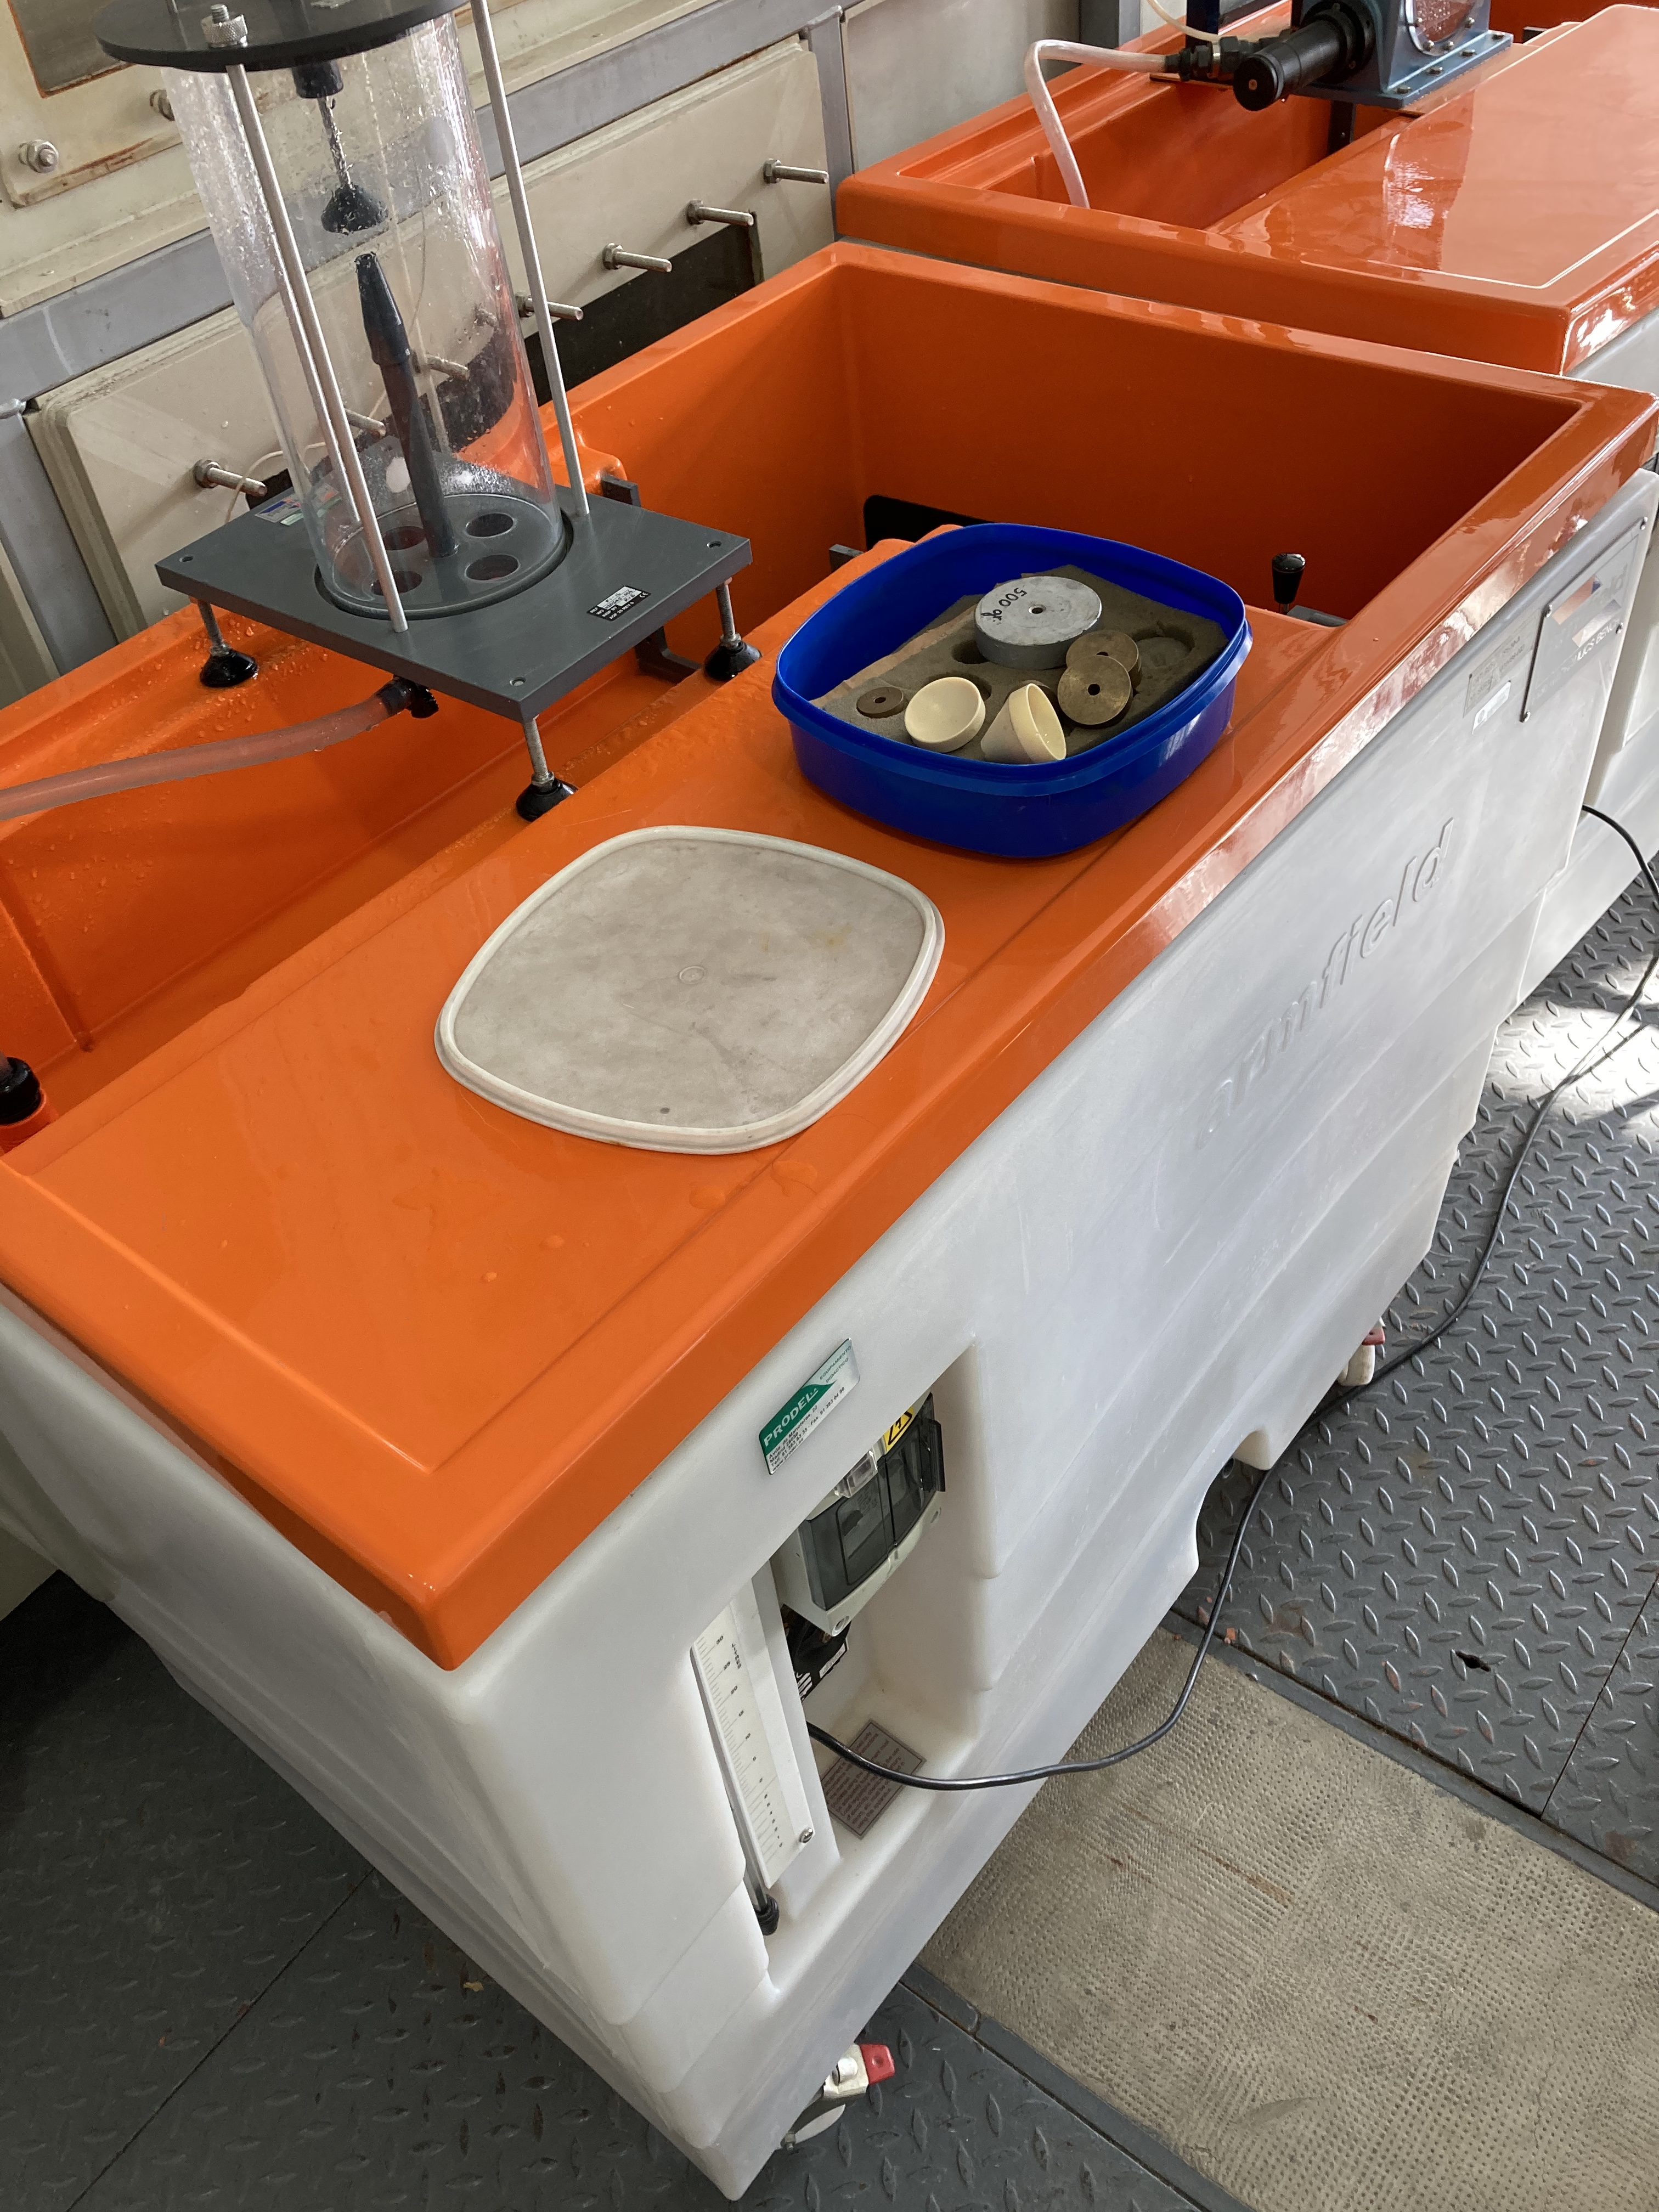
\includegraphics[width=\linewidth]{fotos/aparato_4}
\caption{Dispositivo experimental para la medida de la fuerza que produce un chorro de agua cuando incide sobre un superficie.}
\label{fig9}
\end{minipage}
\hspace{0.5cm}
\begin{minipage}[b]{0.4\linewidth}
\centering
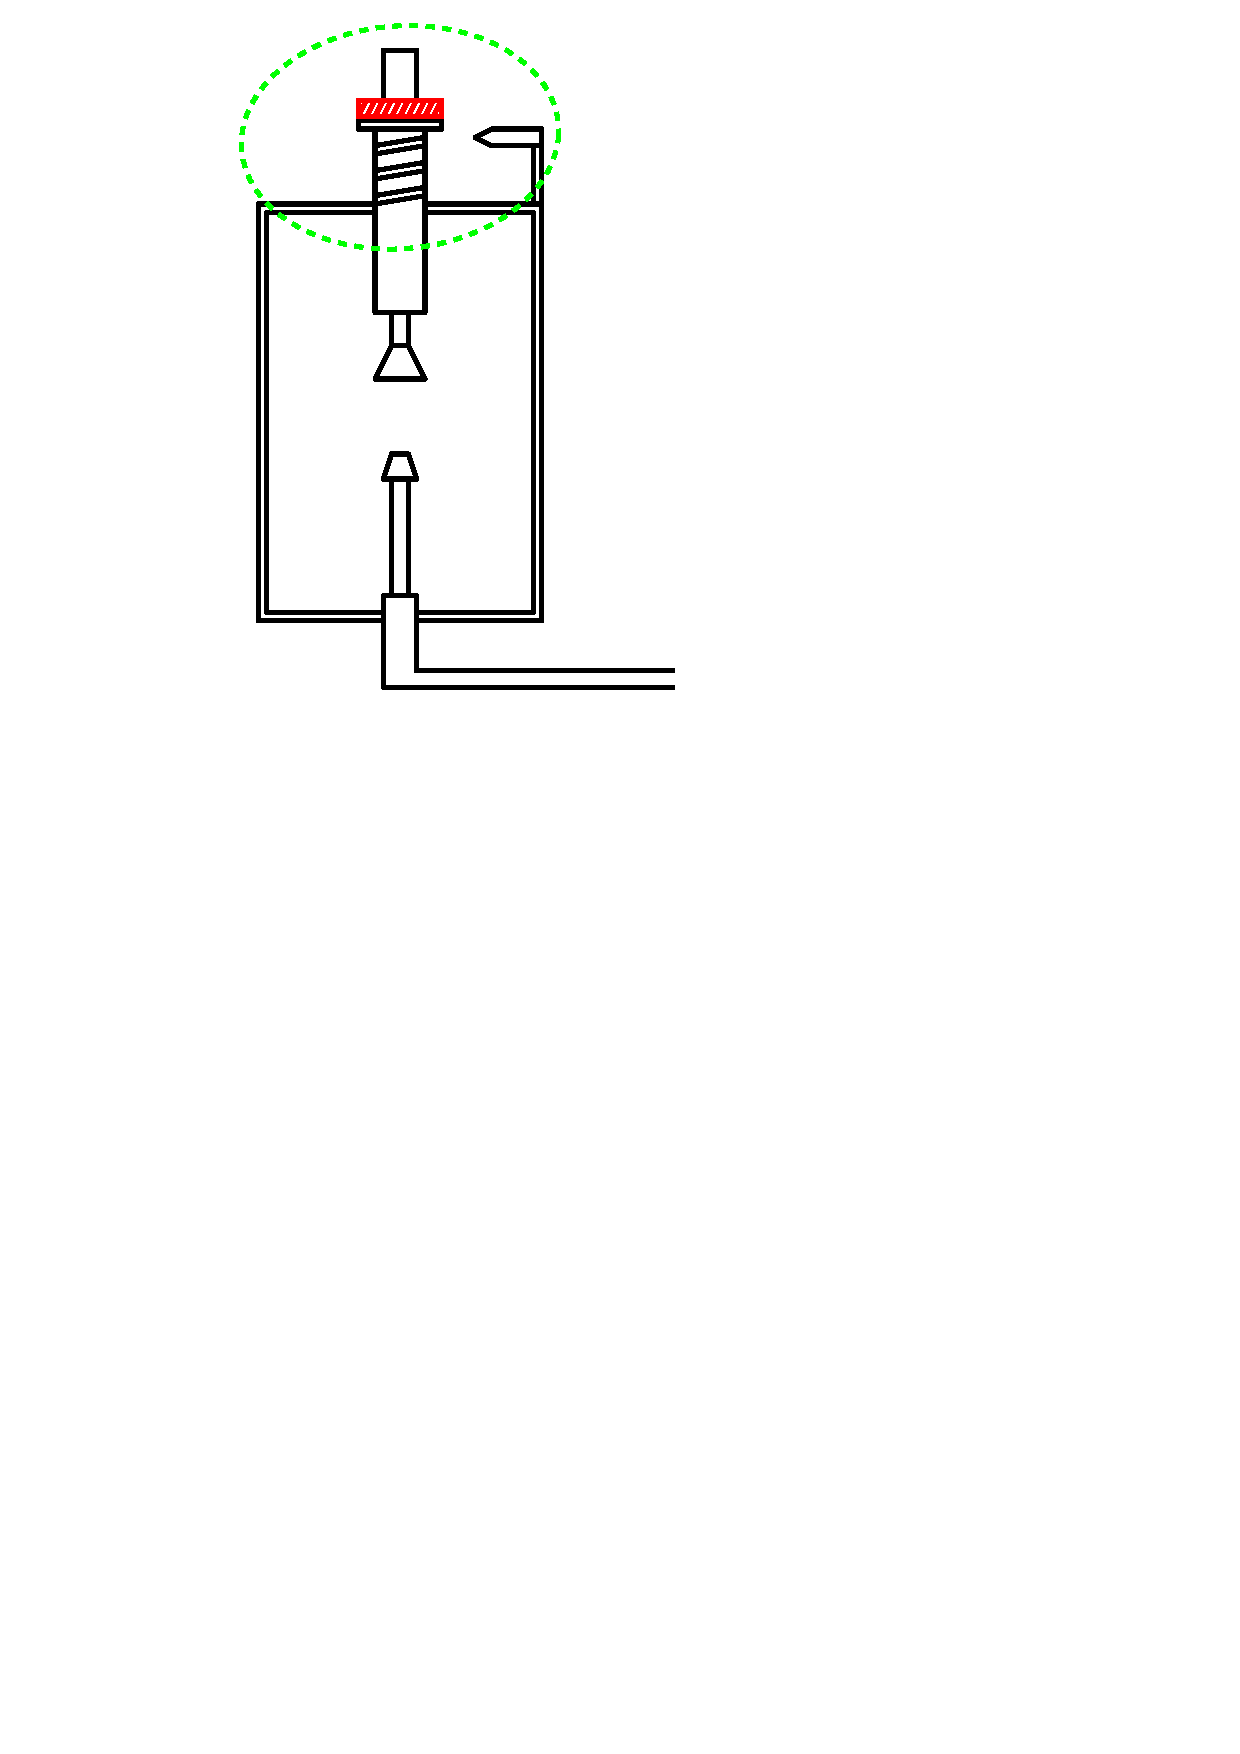
\includegraphics[width=\linewidth]{fotos/esquema_4}
\caption{Esquema del sistema de medición. La parte señalada en verde es la que no es posible apreciar en la figura \ref{fig9}. La zona rayada en rojo representa las pesas que pueden añadirse hasta compensar la fuerza del chorro.}
\label{fig10}
\end{minipage}
\end{figure}

En la figura \ref{fig9} podemos ver un depósito de agua de color blanco. Toda la cubierta naranja hace de tapadera de dicho depósito. En la parte superior podemos ver una plataforma grisácea que soporta firmemente un depósito transparente cilíndrico y dentro del cual vemos una boquilla (que será por donde se impulse el agua) y una superficie deflectora (en el caso concreto de la imagen, está dispuesta a $90\grad$. Las paredes transparentes del cilindro nos permiten ver el proceso y evitan también que nos mojemos durante el experimento.

\begin{wrapfigure}{l}{0.44\textwidth}
\vspace{-0.55cm}
 	 \begin{center}
  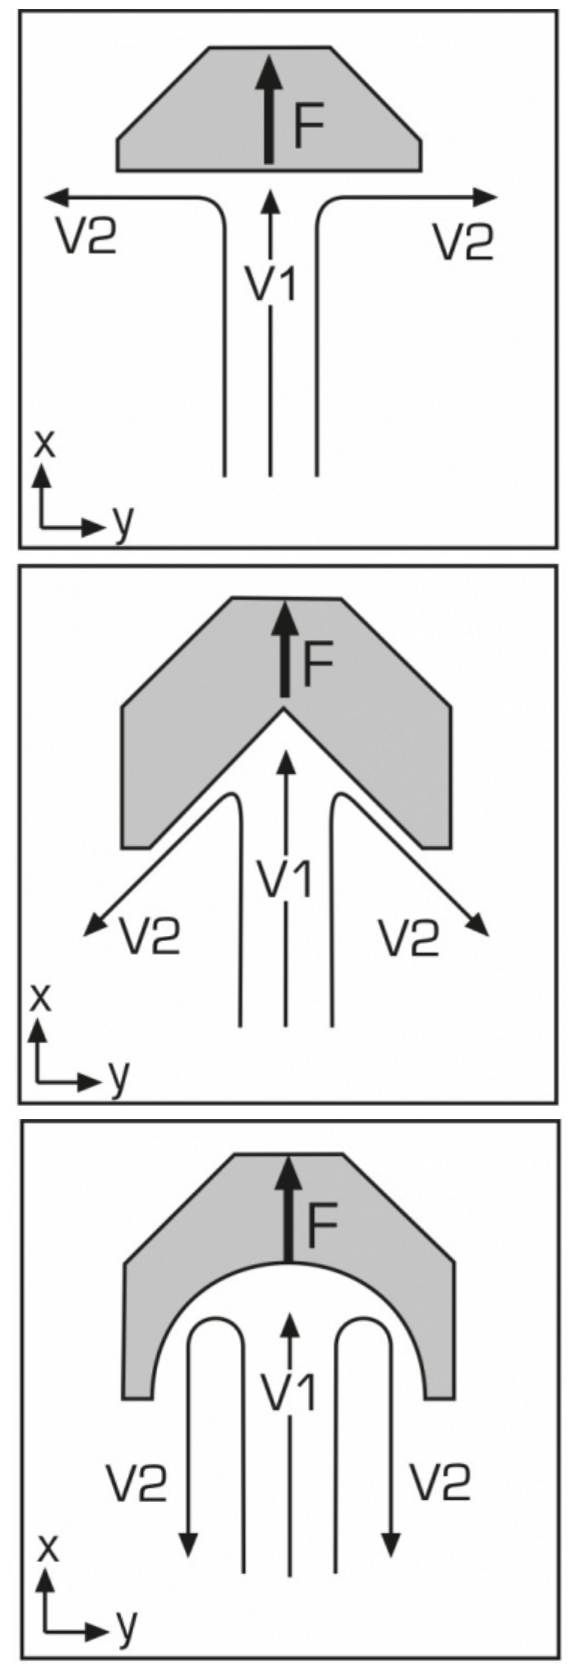
\includegraphics[width=0.42\textwidth]{fotos/deflectores}
  	 \end{center}
  	 \vspace{-0.55cm}
  	\caption[]{Esquema de deflexión del chorro segun superficie deflectora. En nuestro caso la superficie está a $90\grad$, la primera imagen. Fuente de la imagen a pie de página.\footnotemark }
  	\label{fig11}
\end{wrapfigure}
Es importante hacer notar que en la imagen no aparece un elemento fundamental y que se ilustra con un esquema en la figura \ref{fig10}, nos referimos al sistema de medición, con el cual equilibraremos la fuerza del chorro con unos pesos que se irán disponiendo sobre un muelle según aumentemos la presión del chorro de agua.

\footnotetext{ { \scriptsize Enlace a la página web: \url{https://www.gunt.de/es/productos/mecanica-de-fluidos/principios-fisicos/fundamentos-de-la-hidrodinamica/medicion-de-fuerzas-ejercidas-por-un-chorro/070.15008/hm150-08/glct-1:pa-150:ca-778:pr-555}}}

En el experimento tenemos tres fuerzas: la del chorro del agua hacia arriba cuando incide sobre la placa (que llamaremos $F$), la del muelle (que llamaremos $F_{e}$) y la del peso situado en la parte superior (que será $W$). El equilibro puede expresarse como:
\begin{align*}
F=F_{e}+W
\end{align*}

Para simplicar el experimento, es posible eliminar el efecto del muelle realizando el equilibrio de forma que el muelle permanezca siempre en su longitud natural. Y esto podemos lograrlo gracias al indicador de nivel situado junto al muelle.\\

Por otro lado, vamos a estudiar la fuerza del chorro del agua y cómo deflecta en su impacto contra la placa.

En las imágenes de la figura \ref{fig11} puede observarse dos chorros, el incidente y el deflectado. Por el teorema de la cantidad de movimiento según el eje vertical:
\begin{align*}
\sum F_{y}= \frac{dp_y}{dt}
\end{align*}
La cantidad de movimiento se expresa como masa por velocidad, con lo que su derivada será masa por aceleración, en mecánica de fluidos podemos expresar esto como el gasto másico ($kg/s$) por la velocidad ($m/s$), es decir newtons ($N=\frac{kg{\cdot}m}{s^2}$):
\begin{align*}
- F =& G_{sale} \cdot v_{y,sale} - G_{entra}\cdot v_{y,entra}
\end{align*}

El gasto másico es a su vez la densidad $\rho$ (conocida) por el cuadal $Q$ (que podemos calcular) y como nos hablan de velocidad segun $y$, debemos proyectar la velocidad del chorro deflectado con la vertical. El ángulo que forman lo llamaremos $\theta$, y lo tomaremos menor de $90\grad$ por simplicidad.
\begin{align*}
- F =& \rho Q(v \cos\theta - v)
\end{align*}

Por último, cambiando de signo el paréntesis y expresado la velocidad como el caudal entre el área de la boquilla:
\begin{align*}
\boxed{F = \rho \frac{Q^{2}}{A}(1-\cos\theta)}
\end{align*}

Es importante notar que se ha supuesto la velocidad incidente igual a la deflectada, esto podemos hacerlo bajo las siguientes premisas: el caudal de entrada es el mismo que el de salida por continuidad, las presiones en los chorros incidente y deflectado son iguales a la atmosférica, se ha supuesto movimiento ideal con fricción despreciable y se ha aplicado el teorema de Bernoulli:
\begin{align*}
p+\frac{1}{2}\rho v^2= cte
\end{align*}
que por todo lo anterior nos permite concluir que las velocidades son las mismas.
Antes de concluir, incluimos unos datos para los cálculos posteriores: diámetro de la boquilla $8\,mm$ y densidad del agua $\rho=1000\,kg/m^3$.\\

Finalmente, enlazando la conclusión sobre el equilibrio de fuerzas con la expresión que hemos deducido podemos afirmar que:
\begin{align*}
F=W=\rho \frac{Q^{2}}{A}(1-\cos\theta)
\end{align*}

Acerca del procedimiento: se comienza colocando una pesa sobre el platillo (previamente el encargado habrá dispuesto el deflector correspondiente, en nuestro caso fue el de noventa grados). Se enciende el banco hidráulico que suministra la potencia al chorro de agua. Y regular el cuadal de agua hasta que la fuerza del chorro iguale el peso (que la marca del platillo quede alineada con el indicador). Por otro lado, es necesario medir el cuadal del chorro de agua, esto lo conseguimos gracias al depósito volumétrico que tiene el dispositivo empleado. Este, dispone además, de un medidor de nivel que nos será de gran ayuda. Debemos cronometrar con un reloj o el teléfono móvil el tiempo (recomendable que sea superior a 10 segundos) que se tarda en llenar nuestro depósito un $\Delta V$, de forma que el caudal será simplemente el cociente del volumen entre el tiempo ($m^3/s$).

\subsection*{Resultados}

Se incluye a continuación la tabla con los resultados. En todos los casos las medidas han sido tomadas llenando el depósito. Es necesario comentar que el primer grupo de medidas, con el deflector de $90\grad$ debe haber algún error de toma de medidas, pues no es tolerable un error mayor al $100\%$, y solo en el primer dato ya tenemos ¡un error del $224\%$! Sería muy conveniente repetir dicha práctica. Por otro lado, podemos asegurar que se procedió con la mayor prudencia y atención y que posiblemente el error resida en confundir el nivel del depósito ($5L$ en vez de $10L$) o el tiempo cronometrado ($30$ segundos en vez de $40$). En particular, si el tiempo fuera realmente $30.5$ segundos la velocidad pasa a ser $v=3.26\,m/s$, la fuerza $0.54\,N$ y el error a $83.5\%$, lo cual es un valor más razonable comparado con el valor anterior. Indicar también, que el error mínimo es de un $8.05\%$.

\begin{table}[htbp]
  \centering
    \begin{tabular}{ccccccccc}
    \toprule
    \multicolumn{1}{c}{$\mathbf{\theta}$} & \multicolumn{1}{c}{$\mathbf{m}$} & \multicolumn{1}{c}{$\mathbf{W}$} & \multicolumn{1}{c}{$\mathbf{\Delta V}$} & \multicolumn{1}{c}{$\boldsymbol{\Delta t}$} & \multicolumn{1}{c}{$\boldsymbol{Q}$} & \multicolumn{1}{c}{$\mathbf{v}$} & \multicolumn{1}{c}{$\mathbf{F}$} & \multicolumn{1}{c}{$\mathbf{\left|\frac{F-W}{W}\right|}$} \\
    {\small ($grad$)} & {\small ($g$)} & {\small ($N$)} & {\small ($l$)} & {\small ($s$)} & {\small ($l/s$)}& {\small ($m/s$)} & {\small ($N$)} & {\small ($\%$)}\\    
    \midrule
    90 & 100 & 0.98 & 5 & 40.5 & 0.123 & 2.46 & 0.303 & 224 \\
    90 & 200 & 1.96 & 5 & 16.8 & 0.298 & 5.92 & 1.76 & 11.3 \\
    90 & 300 & 2.94 & 5 & 15.9 & 0.314 & 6.26 & 1.97 & 49.6 \\
    90 & 400 & 3.92 & 5 & 12.7 & 0.394 & 7.83 & 3.08 & 27.3 \\
    90 & 500 & 4.91 & 10 & 21.2 & 0.472 & 9.38 & 4.43 & 10.8 \\
    \midrule
    120 & 100 & 0.98 & 5 & 30.1 & 0.166 & 3.31 & 0.824 & 19.1 \\
    120 & 250 & 2.45 & 3 & 10.9 & 0.275 & 5.48 & 2.26 & 8.29 \\
    120 & 400 & 3.92 & 3 & 9.41 & 0.319 & 6.34 & 3.03 & 29.4 \\
    120 & 600 & 5.89 & 3 & 7.14 & 0.420 & 8.36 & 5.27 & 11.7 \\
    120 & 800 & 7.85 & 5 & 10.6 & 0.472 & 9.39 & 6.65 & 18.0 \\
    \midrule
    180 & 200 & 1.96 & 3 & 14.2 & 0.212 & 4.21 & 1.79 & 9.86 \\
    180 & 400 & 3.92 & 5 & 16.6 & 0.302 & 6.01 & 3.63 & 8.05 \\
    180 & 800 & 7.85 & 5 & 10.1 & 0.498 & 9.90 & 9.85 & 20.3 \\
    \bottomrule
    \end{tabular}
  \caption{Resultados experimentales. Notar que se ha añadido una columna adicional con el peso de las masas, de esta forma resulta más fácil comparar la fuerza del chorro y el peso simultáneamente.}
  \label{tab4}
\end{table}

\begin{figure}[H]
 	 \begin{center}
  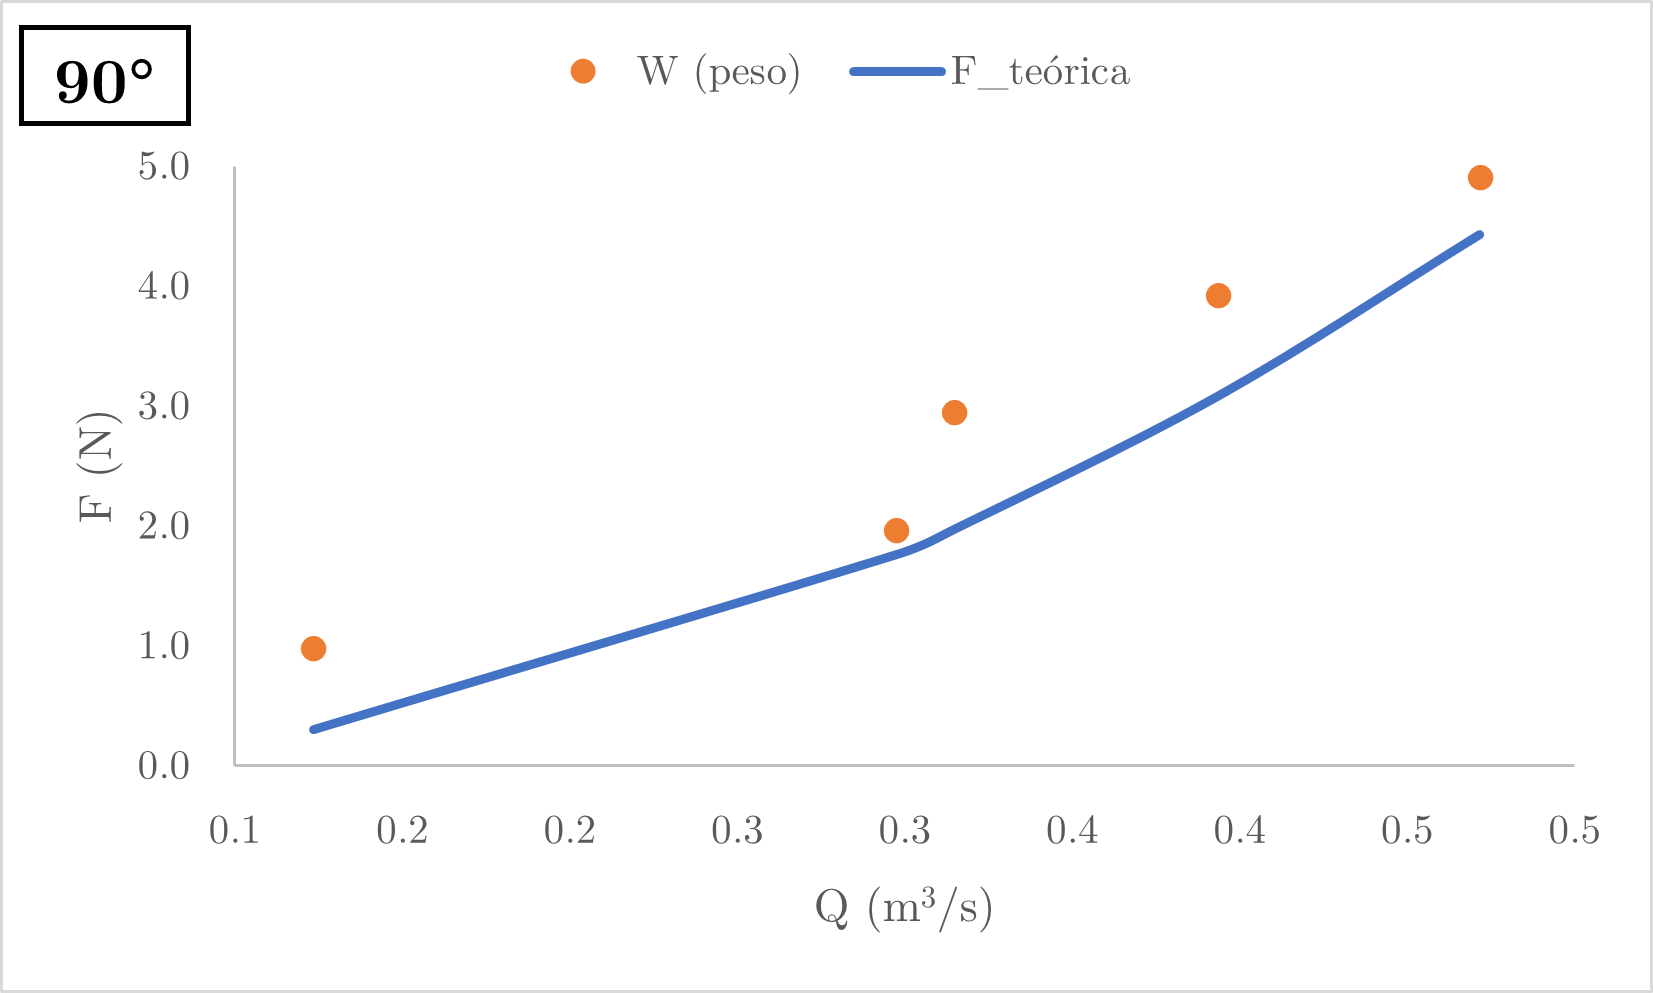
\includegraphics[width=0.9\textwidth]{fotos/Picture1}
  	 \end{center}
  	 \vspace{-0.3cm}
  	\caption{Fuerza teórica y peso ($W$) frente al caudal ($Q$). Para el deflector de $90\grad$.}
  	\label{fig12}
  	\vspace{-0.2cm}
\end{figure}

\begin{figure}[H]
 	 \begin{center}
  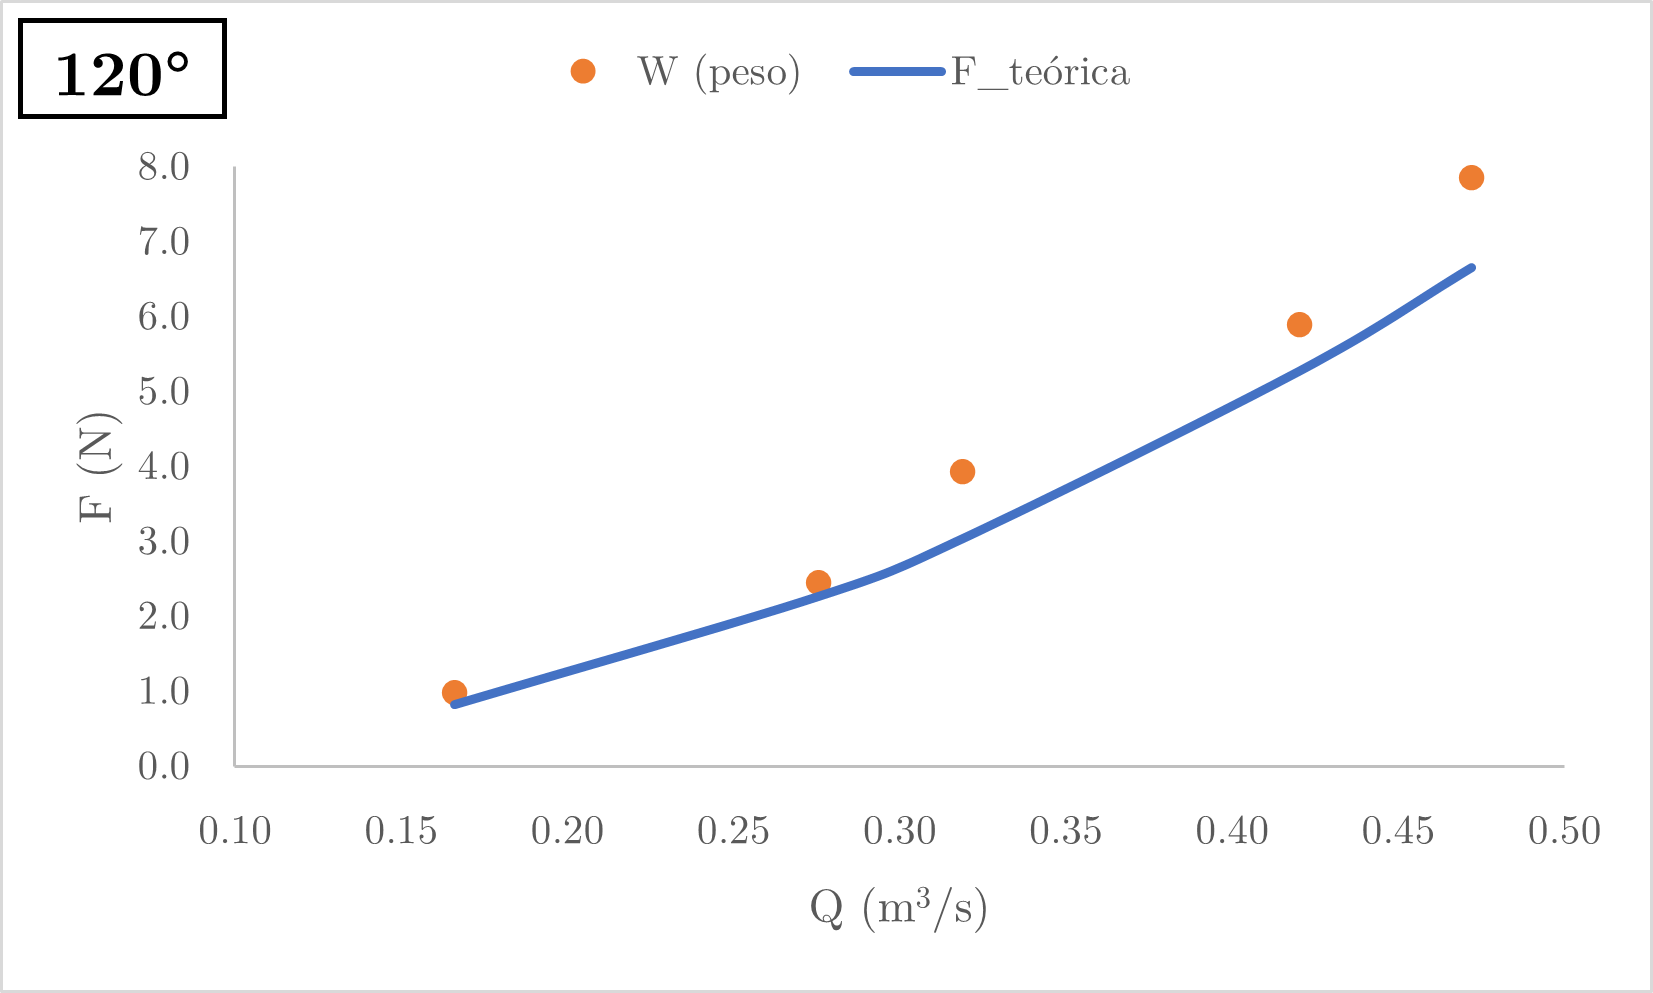
\includegraphics[width=0.9\textwidth]{fotos/Picture2}
  	 \end{center}
  	 \vspace{-0.3cm}
  	\caption{Fuerza teórica y peso ($W$) frente al caudal ($Q$). Para el deflector de $120\grad$.}
  	\label{fig13}
  	\vspace{-0.2cm}
\end{figure}

\begin{figure}[H]
 	 \begin{center}
  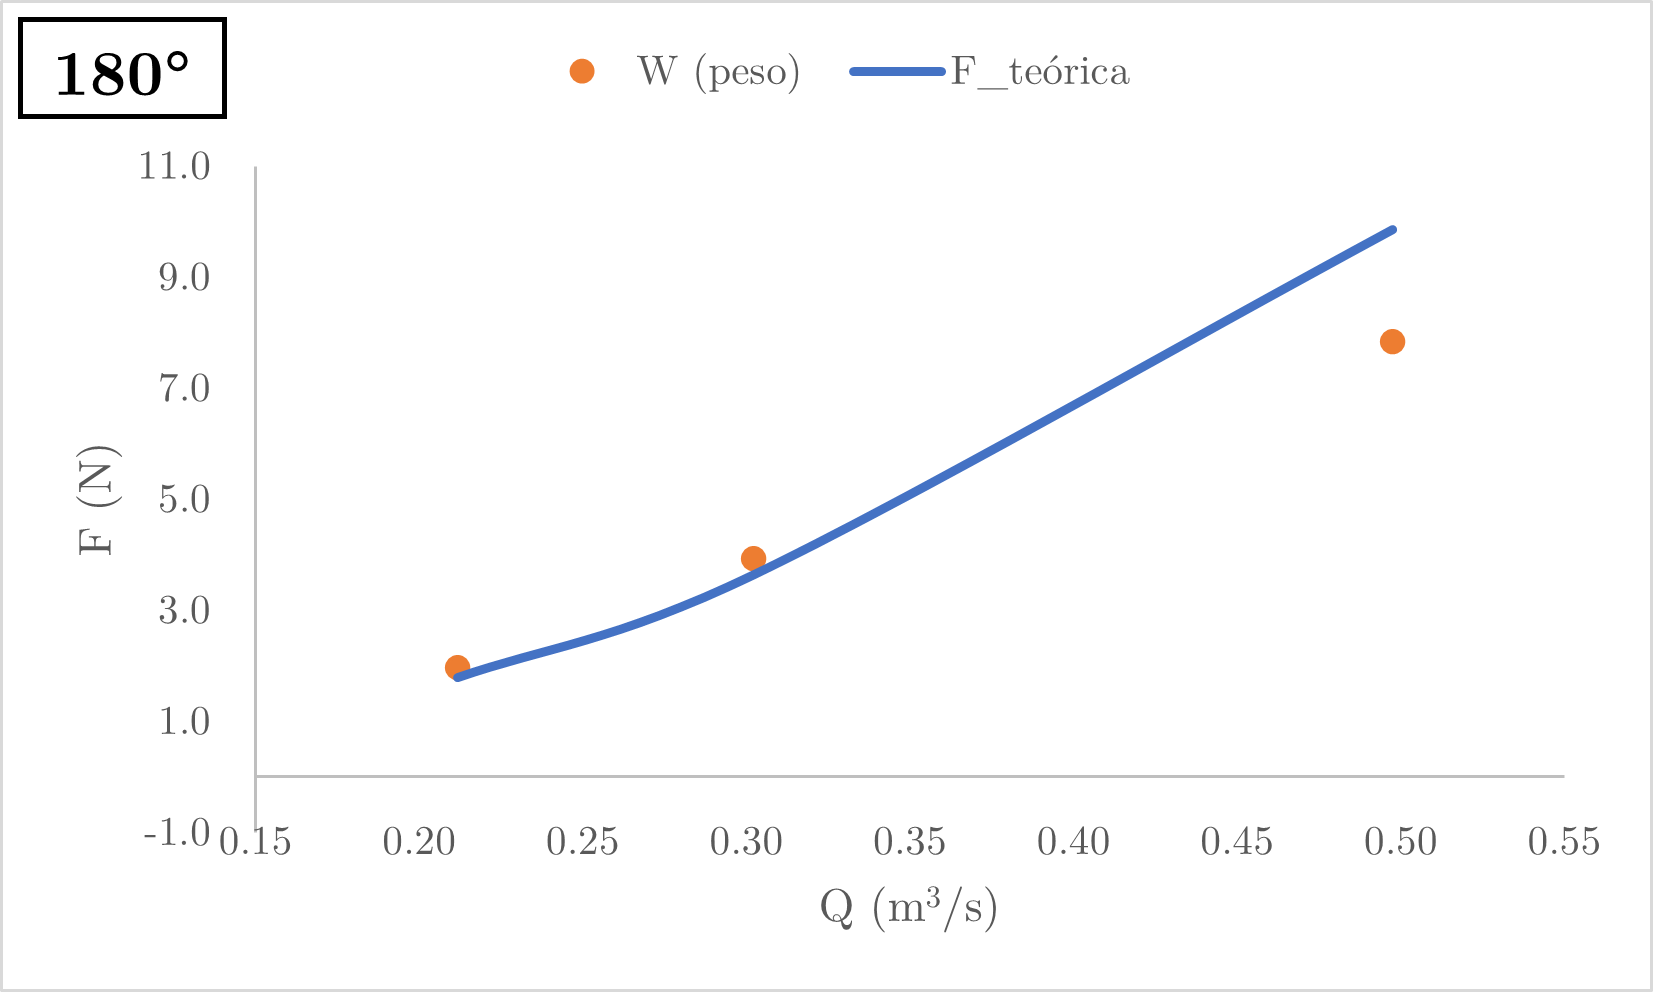
\includegraphics[width=0.9\textwidth]{fotos/Picture3}
  	 \end{center}
  	 \vspace{-0.3cm}
  	\caption{Fuerza teórica y peso ($W$) frente al caudal ($Q$). Para el deflector de $180\grad$.}
  	\label{fig14}
  	\vspace{-0.2cm}
\end{figure}

A la vista de las gráficas anteriores podemos concluir que esta práctica tiene almacenados muchos errores. Creemos que la propagación de estos es debida a que gran parte de la toma de medidas requiere del factor humano, el cual, a este nivel suele cometer muchos y grandes errores. Citamos, por ejemplo, el cálculo del caudal. Para conseguirlo, es necesario iniciar la cuenta del cronómetro mientras se observa la lectura del medidor de nivel del depósito y de la misma forma para la parada del cronómetro; y esto además, entre dos personas, lo cual puede suponer más error en ciertos casos. 

En definitiva, no es sencillo el experimento realizado. Creemos que mejorar el sistema de medición del equilibrado de fuerzas ayudaría mucho. Esto podría realizarse acercando más el indicador de nivel al platillo.

\end{document}